\documentclass[letterpaper,11pt]{article}

%\pdfoutput=1
%\RequirePackage{mathrsfs,mathtools,latexsym,enumerate,framed,enumerate,bbm,appendix,soul}
% \RequirePackage{pdftricks} % throws warnings if used
%\RequirePackage{romanbar}
%\RequirePackage{MnSymbol} 
%\RequirePackage{multirow,mathtools,latexsym, mathrsfs,framed,listings,mleftright,enumitem}

\RequirePackage{amsmath, amsthm, amssymb, mathtools}
\RequirePackage{comment}
\RequirePackage{graphicx}
\RequirePackage{fancyvrb}
\RequirePackage[usenames,dvipsnames,svgnames,table]{xcolor}
    \definecolor{linkcolor}{RGB}{0,0,128}
\RequirePackage[pdfpagelabels,plainpages=false,hypertexnames=true,colorlinks=true,linkcolor=linkcolor,anchorcolor=linkcolor,citecolor=linkcolor,filecolor=linkcolor,menucolor=linkcolor,runcolor=linkcolor,urlcolor=linkcolor,pdfborder={0 0 0}]{hyperref}
\RequirePackage[scale=0.95]{sourcecodepro}
\RequirePackage{mathpazo}
\renewcommand{\baselinestretch}{1.1}
\RequirePackage{dsfont}
\RequirePackage{parskip}
\RequirePackage{tikz}
    \usetikzlibrary{positioning}
\RequirePackage[backend=biber,backref=true,style=numeric,giveninits=true,natbib=true,maxbibnames=12]{biblatex}
    \addbibresource{all.bib}
\RequirePackage{microtype}

\tolerance=800
\hbadness=800

% \setlength{\paperheight}{9in}
% \setlength{\paperwidth}{6in}
% \pdfpagewidth=\paperwidth
% \pdfpageheight=\paperheight

\setlength{\textwidth}{6.5in}
\setlength{\textheight}{9in}
\setlength{\oddsidemargin}{0in}
\setlength{\evensidemargin}{0in}
\setlength{\topmargin}{-0.5in}    


\theoremstyle{plain}% default
\newtheorem{prototheorem}{Theorem}
\newtheorem{theorem}[prototheorem]{Theorem}
\newtheorem{lemma}[prototheorem]{Lemma}
\newtheorem{proposition}[prototheorem]{Proposition}
\newtheorem{corollary}[prototheorem]{Corollary}
%\newtheorem{definition}[prototheorem]{Definition}
%\newtheorem{remark}[prototheorem]{Remark}


\theoremstyle{remark}
\newtheorem{definition}{Definition}
\newtheorem{remark}{Remark}
\newtheorem{assumption}{Assumption}

\DeclarePairedDelimiter\ceil{\lceil}{\rceil}
\DeclarePairedDelimiter\floor{\lfloor}{\rfloor}
\DeclarePairedDelimiter\set{\{}{\}}
\newcommand{\norm}[1]{\left\lVert#1\right\rVert}
\newcommand{\R}{\mathbb{R}}
\newcommand{\prb}{\mathbb{P}}
\newcommand{\ev}[1]{\mathbb{E} \left[ #1 \right]}
\newcommand{\evsub}[2]{\mathbb{E}_{#1} \left[ #2 \right]}
\newcommand{\var}[1]{\text{Var} \left( #1 \right)}
\newcommand{\sigf}{\mathcal{F}}
\DeclarePairedDelimiter{\abs}{\lvert}{\rvert}
\newcommand{\dd}{\, \text{d}}
\newcommand{\eps}{\varepsilon}
\newcommand{\differential}{D}
\newcommand{\mnorm}[1]{\left\| #1 \right\|} %matrix norm
\newcommand{\Z}{\ensuremath \mathbb{Z}}
\newcommand{\W}{\boldsymbol{\mathcal{W}}}
\newcommand{\PM}{\ensuremath \mathcal{P}}
\newcommand{\J}{\mathrm{Couplings}}
\newcommand{\law}{\operatorname{Law}}
\newcommand{\opnorm}[1]{\left\| #1 \right\|_{\mathsf{op}}} 
\newcommand{\wnorm}[1]{\left\| #1 \right\|_{\mathsf{w}}} 
\newcommand{\wonenorm}[1]{\left\| #1 \right\|_{\mathsf{w},1}} 

\newcommand{\twonorm}[1]{\left|\left| #1 \right|\right|_2}

  
\newcommand{\lb}[1]{{\lfloor #1 \rfloor_h}}
\newcommand{\ub}[1]{{\lceil #1 \rceil_h}}
\newcommand{\rn}[1]{\Romanbar{#1}}

\renewcommand{\topfraction}{1.0}
\renewcommand{\textfraction}{0.0}
\renewcommand{\floatpagefraction}{1.0}

\title{GIST: Gibbs self-tuning for locally  \\ 
adaptive Hamiltonian Monte Carlo}
\author{Nawaf Bou-Rabee\thanks{Department of Mathematical Sciences, Rutgers University, \href{mailto:nawaf.bourabee@rutgers.edu}{\texttt{nawaf.bourabee@rutgers.edu}}}
\and
Bob Carpenter\thanks{Center for Computational Mathematics, Flatiron Institute, \href{mailto:bcarpenter@flatironinstitute.org}{\texttt{bcarpenter@flatironinstitute\\.org}}}
\and
Milo Marsden\thanks{Department of Mathematics, Stanford University, 
\href{mailto:mmarsden@stanford.edu}{\texttt{mmarsden@stanford.edu}}}
}

\begin{document}

\maketitle
\begin{abstract}
\noindent
We present a novel and flexible framework for localized tuning of Hamiltonian Monte Carlo samplers by sampling the algorithm's tuning parameters conditionally based on the position and momentum at each step. For adaptively sampling path lengths, we show that randomized Hamiltonian Monte Carlo, the No-U-Turn Sampler, and the Apogee-to-Apogee Path Sampler all fit within this unified framework as special cases.  The framework is illustrated with a simple alternative to the No-U-Turn Sampler for locally adapting path lengths.
\end{abstract}

%\paragraph{Keywords} Markov chain Monte Carlo, Hamiltonian Monte Carlo, Self-Tuning, High Dimensions


\section{Introduction}

Tuning the parameters of Markov chain Monte Carlo (MCMC) algorithms is critical to their  performance, but notoriously difficult in practice.  This challenge is particularly acute for Hamiltonian Monte Carlo (HMC), where the tuning of path length (integration time) \cite{HoGe2014,BoSa2017,betancourt2017conceptual,kleppe2022connecting}, step length (time discretization parameter) \cite{BePiRoSaSt2013,betancourt2014optimizing,biron2024automala}, and pre-conditioner (mass matrix) \cite{GiCa2011,kleppe2016adaptive,whalley2024randomized}~frequently presents a complex trade-off between computational cost and mixing.   The successful self-tuning of path length provided by the No-U-Turn Sampler (NUTS) has led to its widespread adoption as the default sampler in probabilistic programming languages \cite{carpenter2016stan,salvatier2016probabilistic,nimble-article:2017,ge2018t,phan2019composable}.

In NUTS, the path length is adaptively sampled according to U-turn avoiding conditions, which roughly speaking stop the underlying Hamiltonian trajectory whenever it doubles back \cite{HoGe2014,betancourt2017conceptual}. The main idea is to numerically integrate Hamilton's equations forward and backward in time until a U-turn occurs.\footnote{A U-turn must occur in a proper density, but in practice, a cap such as 1024 iterations is imposed.}  A point along this path is then randomly selected such that: (i) the resulting sampler has the correct invariant distribution; and (ii) points far from the starting point are more likely to be selected.  %While originally based on a slice sampler, the latest version of NUTS is based on a multinomial procedure \cite[Appendix A]{betancourt2017conceptual}.  The correctness and basic properties of NUTS have been the subject of several recent works \cite{andrieu2020general, durmus2023convergence}.   

Can the algorithm's other tuning parameters  be similarly self-tuned?   Motivated by the benefits of NUTS, this paper addresses this question by presenting a new framework for adaptively sampling HMC tuning parameters such as  path length, step length, pre-conditioner, etc.\footnote{The approach presented here could also be applied to Metropolis samplers other than HMC.}  This framework is termed Gibbs self-tuning HMC or GIST for short.  In the context of adaptively sampling path lengths,  we demonstrate that GIST includes as special cases almost all locally adaptive HMC samplers in current use including randomized HMC \cite{BoSa2017,BoEb2022}, NUTS \cite{HoGe2014,betancourt2017conceptual}, and the Apogee-to-Apogee Path Sampler \cite{SherlockUrbasLudkin2023Apogee}.  Owing to its simplicity and generality, GIST can be naturally extended to adapting the algorithm's remaining tuning parameters including step size and mass matrix.

To be sure, the primary contribution of this paper is the GIST sampler, which admits a relatively simple proof of correctness.  Moreover, we demonstrate the utility of the GIST sampling framework as a theoretical tool by unifying the proofs of correctness for existing locally adaptive HMC samplers and as a practical tool by developing a novel alternative for locally adapting path lengths.

The remainder of the paper is organized as follows.  
Section~\ref{sec:sthmc} presents the GIST sampling framework for  self-tuning HMC samplers.  In the context of adaptively sampling path lengths, Section~\ref{sec:pathlength} considers some fundamental special cases of  GIST samplers including randomized HMC (Section~\ref{ex:exact_rHMC}), NUTS (Section~\ref{sec:NUTS}), and the Apogee-to-Apogee Path Sampler (Section~\ref{sec:Apogee-to-Apogee}).  Section~\ref{sec:nealsexample} compares GIST samplers for path-length adaptation in the continuous-time context applied to a truncation of an infinite-dimensional Gaussian target measure.  Section~\ref{sec:step-distro} considers path-length adaptation in the discrete-time context, and presents several concrete proposals for sampling the number of leapfrog steps based on the current position and momentum given a fixed step size and mass matrix.  Section~\ref{sec:experiments} describes a novel sampler for adapting path lengths along with experimental evaluation and an empirical comparison to NUTS.

\begin{figure}[t]
\begin{flushleft}
$\textbf{GIST}(\theta)$
\vspace*{2pt}
\hrule
\vspace*{2pt}
\begin{tabular}{ll}
$\theta \in \mathbb{R}^d$ & position
\\
$\rho \in \mathbb{R}^d$ & momentum
\\
$\alpha \in \mathcal{A}$ & algorithm tuning parameter
\end{tabular}
\vspace*{4pt}
\hrule
\vspace*{8pt}
{\footnotesize (INITIALIZE)} \\[2pt]
$\theta_0 = \theta$
\\[12pt]
{\footnotesize (GIBBS)} \\[2pt]
 $\rho_0 \sim \textrm{normal}(0, \textrm{I}_{d \times d})$ \hfill (complete momentum refreshment)
\\[4pt]
$\alpha \sim p(\cdot \mid \theta_0, \rho_0)$ \hfill (sample tuning parameter)
\\[12pt]
{\footnotesize (METROPOLIS-WITHIN-GIBBS)} \\[2pt]
 $(\theta^*, \rho^*) = F(\alpha)(\theta_0, \rho_0)$ \hfill (compute proposal)
\\[4pt]
$u \sim \textrm{uniform}([0, 1])$ 
\\[4pt]
if $u < e^{-\Delta H(\theta_0,\rho_0)} \, \dfrac{p\left( \pi(\theta_0, \rho_0)(\alpha) \, | \, \mathcal{S} \circ F(\alpha)(\theta_0, \rho_0) \right)}{p \left(\alpha\, | \, \theta_0, \rho_0 \right)} $  \\
\null \quad return $\theta^*$ \hfill (accept) 
\\[6pt]
else \\[-6pt]
\null \quad return $\theta_0$ \hfill (reject)
\vspace*{4pt}
\hrule
\caption{\it {\bfseries  GIST Sampling}.  The GIST sampler differs from standard HMC in the sampling of the tuning parameter and subsequent adjustment of the acceptance probability.  Here we use the shorthand $\Delta H(\theta, \rho) := H \circ F(\alpha)(\theta,\rho) - H(\theta, \rho)$ and $\emph{I}_{d \times d}$ denotes the $d \times d$ identity matrix.}
\label{fig:general-self-tuning-step}
\end{flushleft}
\end{figure}

\section{A framework for self-tuning Hamiltonian Monte Carlo}

\label{sec:sthmc}

Hamiltonian Monte Carlo (HMC) is a class of MCMC methods for sampling absolutely continuous probability target distributions of the form 
\begin{equation} \label{eq:target}
\mu(d\theta, d\rho) \propto e^{-H(\theta,\ \rho)} \, m( d\theta \, d\rho) \;, 
\end{equation}
which have a density relative to Lebesgue measure $m$ on phase space $\mathbb{R}^{2d}$, with position $\theta \in \mathbb{R}^d$ and momentum $\rho \in \mathbb{R}^d.$  For simplicity, we assume  the case of a separable Hamiltonian function with unit mass matrix, i.e., \[
H(\theta,\rho) = U(\theta) + \frac{1}{2} \, \rho^{\top} \, \rho \;, 
\]
for a continuously differentiable potential energy function $U: \mathbb{R}^d \to \mathbb{R}$ such that $\int e^{-U(\theta)} d\theta < \infty$.   The non-normalized target density of interest is $e^{-U(\theta)}$ for model parameters $\theta.$

A defining ingredient of any HMC algorithm is a reversible, volume-preserving map $F(\alpha): \mathbb{R}^{2d} \to \mathbb{R}^{2d}$ where $\alpha$ encapsulates the algorithm tuning parameters.  This map is typically obtained from discretizing Hamilton's equations for the Hamiltonian function $H(\theta,\rho)$, i.e.,  \[
\frac{d}{dt} \theta_t = \rho_t \;, \quad \frac{d}{dt} \rho_t = - \nabla U(\theta_t) \;. 
\] Reversibility and volume-preservation ensure that the map $F(\alpha)$ is Metropolis adjustable \cite{BoSaActaN2018}.  Note that $\mathcal{S} \circ F(\alpha)$ is a volume-preserving involution where $\mathcal{S}: \mathbb{R}^{2d} \to \mathbb{R}^{2d}$ is the momentum flip map defined by $\mathcal{S}(\theta, \rho) = (\theta, -\rho)$ for all $(\theta, \rho) \in \mathbb{R}^{2d}$ \cite{Hairer2010GeometricNumerical}.  We suppose that the tuning parameter $\alpha$
takes values in a set $\mathcal{A}$ where $(\mathcal{A}, \mathcal{B}, \eta)$ is a measure space with $\sigma$-algebra $\mathcal{B}$ and background measure $\eta$.  

To ``self tune''  the parameter $\alpha$, the state space $\mathbb{R}^{2d}$ is enlarged to a product space $\mathbb{R}^{2d} \times \mathcal{A}$. On this enlarged space, an enlarged target measure is defined by specifying a conditional distribution of the tuning parameter $\alpha$ given the position and momentum $(\theta, \rho)$, i.e.,  \begin{equation} \label{eq:enlarged_target}
\mu_e(d\theta, d\rho, d\alpha) \propto  e^{-H(\theta, \rho)} \, p( \alpha \, | \, \theta, \rho) \, (m \otimes \eta) (d\theta \, d\rho  \, d\alpha) \;.
\end{equation}  Note that the $(\theta, \rho)$-marginal of $\mu_e$ is the desired target measure $\mu$.  Explicit forms of the conditional distribution $p( \alpha \, | \, \theta, \rho)$ are specified in subsequent sections for the case of path length adaptivity.  


For any position and momentum $(\theta, \rho) \in \mathbb{R}^{2d}$, let $\pi(\theta, \rho) : \mathcal{A} \to \mathcal{A}$ be a measurable map acting on the  tuning parameter $\alpha \in \mathcal{A}$ such that \begin{equation}
 \label{eq:G}
 G: (\theta, \rho, \alpha) \mapsto \Big( S \circ F(\alpha)(\theta, \rho), \, \pi(\theta, \rho)(\alpha) \Big) 
\end{equation} is a $(m \otimes \eta)$-preserving involution on $\mathbb{R}^{2d} \times \mathcal{A}$.   This clearly holds when the map $\pi(\theta, \rho)$ is taken to be the identity map on $\mathcal{A}$.

In terms of this notation, Figure~\ref{fig:general-self-tuning-step} describes a transition step of the ``GIST'' (Gibbs self-tuning HMC) sampler.  The following theorem indicates that the GIST sampler is correct.  
\begin{theorem} \label{thm:correctness}
The GIST sampler in Figure~\ref{fig:general-self-tuning-step} generates a Markov Chain $\theta_0, \theta_1, \dots $ on $\mathbb{R}^d$ that is reversible with respect to $e^{-U( \theta) } m(d \theta)$.
\end{theorem}


A detailed, self-contained proof of Theorem~\ref{thm:correctness} is provided in Appendix~\ref{app:proof_of_correctness}. By interpreting the GIST sampler as a Gibbs sampler, the proof shows that each update in Figure~\ref{fig:general-self-tuning-step} leaves invariant the enlarged target \eqref{eq:enlarged_target}.  In particular, the accept/reject step is interpreted as a Metropolis-within-Gibbs step on the enlarged space $\mathbb{R}^{2d} \times \mathcal{A}$ with target measure defined in \eqref{eq:enlarged_target}, proposal given by $G$ defined in \eqref{eq:G}, and corresponding acceptance probability \begin{equation} \label{eq:acceptanceprobability}
a_e(\theta_0, \rho_0, \alpha) = 1 \wedge \left(  e^{\displaystyle -\Delta H(\theta_0,\ \rho_0)} \, \dfrac{p\left(\pi(\theta_0, \rho_0)(\alpha) \, | \, \mathcal{S} \circ F(\alpha)(\theta_0, \rho_0) \right)}{ p \left(\alpha\, | \, \theta_0, \rho_0 \right)} \right) \;,
\end{equation} 
where we used the shorthand $\Delta H(\theta, \rho) := H \circ F(\alpha)(\theta,\rho) - H(\theta, \rho)$ for $(\theta, \rho, \alpha) \in \mathbb{R}^{2d} \times \mathcal{A}$.
Note, this Metropolis-within-Gibbs step is correct because we assume that the map $G$ on $\mathbb{R}^{2d} \times \mathcal{A}$ is a $(m \otimes \eta)$-preserving involution; for a detailed justification see Lemma~\ref{lem:DeterministicMetropolization} in Appendix~\ref{app:proof_of_correctness}.

\begin{remark}
Just as the Markov chain for standard HMC can be formulated over phase space variables $(\theta, \rho) \in \mathbb{R}^{2d}$, the Markov chain for GIST can also be formulated over triples $(\theta, \rho, \alpha) \in \mathbb{R}^{2d} \times \mathcal{A}$.  However, in the case treated here of full momentum and tuning parameter refreshment, the sequence of $\theta$ values by itself forms a Markov chain and including the other variables is superfluous.
\end{remark}

\begin{remark}
In addition to adaptively sampling HMC tuning parameters, the GIST sampler can also be applied to randomize the time integrator for the Hamiltonian flow, as in \cite{BouRabeeMarsden2022,BouRabeeKleppe2023}.  In this case, the tuning parameter would specify a particular time integrator within a parametric family of time integrators that are each reversible and volume-preserving.  In certain representative models, randomized time integrators have provably better complexity for Hamiltonian MCMC than the frequently used leapfrog integrator \cite{shen2019randomized,ErgodicityRMMHYB,Cao_2021_IBC,BouRabeeMarsden2022,BouRabeeSchuh2023B,BouRabeeOberdoerster2023}.  
\end{remark}

\section{Adaptively sampling path lengths}\label{sec:pathlength}

To make the GIST sampling framework more concrete and demonstrate its breadth, this section shows that several fundamental HMC samplers that locally adapt path lengths fit within this unified framework.  

\subsection{Sampling path lengths in randomized HMC}\label{ex:exact_rHMC}

In randomized forms of HMC, the path length or the step length is generated randomly at each iteration independently of the current position and momentum \cite{Ma1989}; using, e.g., an exponential distribution over path length \cite{BoSa2017,BoEb2022}, an empirically learned distribution over path length \cite{wu2018faster}, or a uniform distribution over path and step lengths \cite{Ma1989,Ne2011}.  These can all be analyzed as instances of the GIST sampler given in Figure~\ref{fig:general-self-tuning-step}.  

As an example, consider $F(\alpha)(\theta, \rho) = \varphi_\alpha(\theta, \rho)$ where we have introduced the exact Hamiltonian flow $\varphi_{\alpha}: \mathbb{R}^{2d} \to \mathbb{R}^{2d}$ at time $\alpha \ge 0$. Take $\mathcal{A} = [0, \infty)$ and $\eta$ to be the Lebesgue measure on $\mathbb{R}$. Define $p(\alpha \mid \theta, \rho) = \lambda e^{- \lambda \alpha}$ where $\lambda > 0$; that is, $\alpha$ is an exponential random variable with parameter $\lambda$.  In this case, the map $G$ in \eqref{eq:G} is given explicitly by $G : (\theta, \rho, \alpha) \mapsto ( \mathcal{S} \circ F(\alpha)(\theta, \rho), \ \alpha)$, for which $a_e \equiv 1$ (the proposal is always accepted), and Figure~\ref{fig:general-self-tuning-step} reduces to a draw from randomized HMC at the first jump time \cite{BoSa2017,BoEb2022}.

The other randomized forms of HMC that generate randomly the tuning parameter independently of the current position and/or momentum can be analyzed in exactly the same way.  In Section~\ref{sec:nealsexample}, in the setting of a truncation of an infinite-dimensional Gaussian measure, the performance of randomized HMC is compared with a GIST sampler that we describe next. 

\subsection{Adapting path lengths in exact HMC}\label{ex:exact_stHMC}

Consider again $F(\alpha) = \varphi_\alpha$ where  $\varphi_{\alpha}: \mathbb{R}^{2d} \to \mathbb{R}^{2d}$ is the exact Hamiltonian flow map at time $\alpha \ge 0$.  Take $\mathcal{A} = [0, \infty)$ and $\eta$ to be the Lebesgue measure on $\mathbb{R}$.  Let $\tau(\theta, \rho):\mathbb{R}^{2d} \to (0, \infty)$ be any measurable function.   Define \[ p(\alpha \mid \theta, \rho) \, = \,  \dfrac{1}{\tau(\theta, \rho)} \mathds{1}_{[0, \ \tau(\theta, \ \rho)]}( \alpha ) \;.
\] That is, conditioned on the position and momentum $(\theta, \rho)$, $\alpha$ is a uniform random variable over the interval  $[0,\tau(\theta, \rho)]$.  Here $\mathds{1}_A$ denotes the standard indicator function of a set $A$.  As a shorthand, let $\tau_1 = \tau(\theta_0, \rho_0)$ and $\tau_2 = \tau(\mathcal{S} \circ \varphi_{\alpha}(\theta_0, \rho_0))$, i.e., the function $\tau$ evaluated at the current state of the chain $(\theta_0, \rho_0)$ and the proposed state but with momentum reversed $\mathcal{S} \circ \varphi_{\alpha}(\theta_0, \rho_0)$.
In this case, the map $G$ in \eqref{eq:G} is given explicitly by \[
G : (\theta, \rho, \alpha) \mapsto ( \mathcal{S} \circ F(\alpha)(\theta, \rho), \ \alpha) \;, 
\] and the corresponding acceptance probability in \eqref{eq:acceptanceprobability} reduces to \[ a_e(\theta_0, \rho_0, \alpha) \, = \, 1 \wedge \left( \frac{\tau_1}{\tau_2} \mathds{1}_{ \{  \tau_2 \geq \alpha \} } \right) \;, \] because $\Delta H(\theta_0, \rho_0) = 0$ for the exact Hamiltonian flow.  The indicator in this Metropolis ratio indicates that  $p(\alpha \mid \mathcal{S} \circ \varphi_{\alpha}(\theta_0, \rho_0)) \ne 0$.

Conditions avoiding U-turns in the exact Hamiltonian flow can be used to specify the function $\tau(\theta, \rho)$.  There are several ways to characterize such $U$-turn conditions. For example, here is a condition based on when the angle between the initial velocity $\rho_0 \in \mathbb{R}^d$ and the velocity $\rho_t \in \mathbb{R}^d$ at time $t \ge 0$ first exceeds $\pi/2$ \begin{equation} \label{eq:ct_angle}
\tau(\theta_0, \rho_0) \ := \ \inf\{ t > 0 ~:~ \rho_0 \cdot \rho_t \le 0 \} \;,
\end{equation} where we have introduced $(\theta_t, \rho_t) := \varphi_t(\theta_0, \rho_0)$ for $t \ge 0$.  Another condition is based on when the squared distance $\Gamma(t) := | \theta_0 - \theta_t|^2$ between the initial configuration $\theta_0 \in \mathbb{R}^d$ and the configuration $\theta_t \in \mathbb{R}^d$ at time $t \ge 0$ first decreases \begin{equation} \label{eq:ct_dist}
\tau(\theta_0, \rho_0) \ := \ \inf\{ t > 0 ~:~ \Gamma'(t) < 0 \} \;.
\end{equation}
These continuous-time U-turn conditions have discrete-time analogs, which are discussed in the next example and Section~\ref{sec:step-distro}.  




\subsection{Adapting path lengths in numerical HMC}\label{sec:numericalHMC}

Fix $h>0$.  Let $\Phi_h: \mathbb{R}^{2d} \to \mathbb{R}^{2d}$ denote one step of the leapfrog integrator with step length $h$.  Consider $F(\alpha) = \Phi_h^{\alpha}$ where $\alpha$ is the number of leapfrog steps. Take $\mathcal{A} = \mathbb{N}$ and let $\eta$ be the counting measure. Similarly to the above, let $\tau: \mathbb{R}^{2d} \to \mathbb{N}$ be a measurable function and define \[ p(\alpha \mid \theta, \rho) = \frac{1}{\tau(\theta, \rho)} \mathds{1}_{\{0,\, \dots, \, \tau(\theta, \, \rho)-1\} }(\alpha) \;.  \]
Similarly to the above, the map $G$ in \eqref{eq:G} is given explicitly by \[
G : (\theta, \rho, \alpha) \mapsto ( \mathcal{S} \circ F(\alpha)(\theta, \rho), \ \alpha) \;,
\] and the corresponding acceptance probability in \eqref{eq:acceptanceprobability} simplifies to \[
a_e(\theta_0, \rho_0, \alpha) \, = \, 
1 \wedge \left( e^{-\Delta H(\theta_0, \rho_0)} \frac{\tau_1}{\tau_2} \mathds{1}_{\{ \tau_2 \geq \alpha \} } \right) \;, \]
where $\tau_1 = \tau(\theta_0, \rho_0)$ and $\tau_2 = \tau(\mathcal{S} \circ \Phi^{\alpha}_h(\theta_0, \rho_0))$.


\subsection{Adapting path lengths in NUTS}\label{sec:NUTS} 

Here we show that NUTS is a special case of the GIST sampler presented in Figure~\ref{fig:general-self-tuning-step}. 

In order to write NUTS as a GIST sampler, we first explain NUTS more precisely following the terminology and framework introduced in \cite{betancourt2017conceptual, durmus2023convergence}.   Given the current position and momentum $(\theta_0, \rho_0) \in \mathbb{R}^{2d}$, the idea behind NUTS is to first randomly generate a finite subset of integers $J \subset \mathbb{Z}$, and in turn, sample the next state of the chain from among the leapfrog iterates $ \{\Phi_h^i(\theta_0, \rho_0) \}_{i \in J}$. Following the notation of \cite{durmus2023convergence}, let $P_h(J \mid \theta_0, \rho_0)$ be the probability of selecting $J$ and let $Q_h(i \mid J, \theta_0, \rho_0)$ be the probability  of selecting the $i$-th leapfrog iterate $\Phi_h^i(\theta_0, \rho_0)$. In \cite{durmus2023convergence}, these are referred to as the ``orbit'' and ``index'' selection kernels, respectively. 

More precisely, the random procedure to generate the set $J$ can be described by induction. First, take $J_{0} = \{ 0 \}$. Then, given $J_k$, we first check whether the leapfrog iterates $\{\Phi_h^i(\theta_0, \rho_0) \}_{i \in J_k}$  satisfy the U-turn condition:
\[\rho_+ \cdot (\theta_+ - \theta_-) < 0 \quad \text{and} \quad \rho_- \cdot (\theta_- - \theta_+) < 0 \]
where $(\theta_+, \rho_+) = \Phi_h^{\max{J_k}}(\theta_0, \rho_0)$ and $(\theta_-, \rho_-) = \Phi_h^{\min J_k}(\theta_0, \rho_0)$. If this condition is met, we output $J = J_k$. If instead no U-turn is encountered, then sample $I_{k+1}$ uniformly from $\{ J_k + |J_k|, J_k - |J_k| \}$. This set is the next proposed extension to the set $J_k$. 

This proposed extension will either be accepted, yielding $J_{k+1} = J_k \cup I_{k+1}$, or rejected, returning $J = J_k$. To ensure the correctness and efficiency of the algorithm the following symmetry condition is imposed: $P_h(J \mid \theta_0, \rho_0) = P_h(J - i \mid \Phi_h^i(\theta_0, \rho_0))$ for all $i \in J$. This condition ensures that the probability of obtaining a particular set of leapfrog iterates $\{\Phi_h^i(\theta_0, \rho_0)\}_{i \in J}$ is uniform with respect to the starting point $\Phi_h^i(\theta_0, \rho_0)$ within this set for all $i \in J$. 

Imposing this constraint will require that some proposed extensions $I_{k+1}$ are rejected. For every $i \in J_k$, corresponds an alternate sequence of extensions $I'_1, \dots, I'_k$ which would have produced the set $J_k - i$ had the orbit generating procedure instead been started at $\Phi_h^i(\theta_0, \rho_0)$.  To enforce $P_h(J \mid \theta_0, \rho_0) = P_h(J-i \mid \Phi_h^i(\theta_0, \rho_0))$, it is sufficient to require that $J_k$ satisfies the No-Intermediate-U-Turn property. This property states that at no stage in this alternate sequence of extensions $I_1', \dots, I_k'$ would the U-turn condition  have been triggered.


%In particular, the set $J_k$ is generated using Bernoulli random variables $\beta_1, \dots, \beta_k$ determining the choices of intermediate sets $I_1, \dots, I_k$ at each stage of this procedure. Moreover, every $i \in J_k$ corresponds bijectively to an equally probable sequence $\beta_1', \beta_2', \dots, \beta_k'$ which would have produced $J_k-i$ starting at $\Phi_h^i(\theta_0, \rho_0)$ and hence the same set of leapfrog iterates.

%In particular, set $\beta_l = I_{I_l = J_l + |J_l|}$ and let $B = \beta_1 + 2\beta_2 + \dots 2^{k-1} \beta_k$. Then, a careful analysis reveals that $J_k = \{0, 1, \dots, 2^k -1\} - B$. Taking instead $\beta_1', \dots, \beta'_k$ to be the binary expansion of i + B would produce J-i. 

%To the alternate sequence $\beta_1', \dots, \beta_k'$  corresponds an alternate sequence of intermediate sets $I_1', \dots, I_k'$. These should be considered as corresponding to an equally probable alternate sequence of intermediate sets of leapfrog iterates which could have been produced had the procedure been started at $\Phi_h^i(\theta_0, \rho_0)$. To show $P_h(J \mid \theta_0, \rho_0) = P_h(J-i \mid \Phi_h^i(\theta_0, \rho_0))$ it is necessary that at every stage $J_k$ satisfies the property that for all $i \in J_k$ at no stage in this alternate sequence $I_1', \dots, I_k'$ would the U-turn condition with starting point $\Phi_h^i(\theta_0, \rho_0)$ have been triggered. For convenience we term this the No-Intermediate-U-Turn property.  %\textbf{Milo - to -Nawaf: Feel free to rename this property or use some other turn of phrase. I just felt it got really confusing to continually write "this property" over and over so that it would be useful to have a name for what I was referring to}

To ensure that every $J_k$ satisfies the No-Intermediate-U-Turn property, we simply need to reject any proposal $I_{k+1}$ where $J_{k+1} = J_k \cup I_{k+1}$ does not satisfy the No-Intermediate-U-Turn property. While naively this appears to involve checking over exponentially many sequences of extensions, this step can be implemented efficiently. Indeed, over different choices of $i \in J_k$ many of the alternate sequences will refer to the same set of leapfrog iterates. Since the U-turn condition depends only on the leapfrog iterates, we therefore need only check that all possible intermediate sets of leapfrog iterates have no U-turns. As the number of possible intermediate sets of leapfrog iterates is relatively small, this observation greatly reduces the complexity of checking the No-Intermediate-U-Turn property. See Remark \ref{rmk:orbit-selection-complexity} for more details about the computational complexity of the orbit generation procedure.

Having generated $J$ using this randomized orbit selection procedure, NUTS then generates $i \in J$ according to the index selection kernel $Q_h(i \mid \theta_0, \rho_0, J)$ and returns $\Phi_h^i(\theta_0, \rho_0)$ as the next state. %In practice, for algorithmic efficiency this sample is generated concurrently with the set $J$, but it is equivalent to describe this as a sequential procedure.
There are two index selection kernels commonly used in practice. The first is given by the Boltzmann weight of the corresponding leapfrog iterate, i.e., $Q_h(i \mid \theta_0, \rho_0, J) \propto e^{-H(\Phi_h^i(\theta_0, \rho_0))} $. The second is biased progressive sampling, as detailed in \cite{betancourt2017conceptual}. 

We are now in position to describe NUTS as a GIST sampler. Let $\mathcal{A} = \mathcal{P}_F \times \mathbb{Z}$ where 
$\mathcal{P}_F = \{J \subset \mathbb{Z} \mid |J|<\infty \}$, let $\eta$ be the counting measure on $\mathcal{P}_F \times \mathbb{Z}$, and write the tuning parameter in components as $\alpha = (J, i) \in \mathcal{A}$. For all $(\theta, \rho, \alpha) \in \mathbb{R}^{2d} \times \mathcal{A}$, define
\[p(J, i \mid \theta, \rho) = P_h(J \mid \theta, \rho) Q_h(i \mid \theta, \rho, J) \;. \]
As in Section \ref{sec:numericalHMC}, let $F(\alpha)(\theta, \rho) = \Phi_h^i(\theta, \rho)$.
The map $G$ given in (\ref{eq:G}) can be written explicitly as
\[G(\theta, \rho, J, i) = (\mathcal{S} \circ \Phi_h^i(\theta, \rho), -(J- i), i) \;.
\]
The resulting GIST sampler in Figure~\ref{fig:general-self-tuning-step} corresponds to NUTS. Notably, the Metropolis-within-Gibbs step for NUTS is always accepted. Indeed, since $\{\Phi_h^i(S(\theta, \rho))\}_{i \in -J} = \{\Phi_h^{-i}(S(\theta, \rho))\}_{i \in J} =\{S(\Phi_h^{i}(\theta, \rho))\}_{i \in J}$ a short coupling construction shows $P_h(-J \mid \mathcal{S}(\theta, \rho)) = P_h(J \mid \theta, \rho)$. Combining this with $P_h(J-i \mid \Phi_h^i(\theta, \rho)) = P_h(J \mid \theta, \rho)$ gives $P_h(-(J-i) \mid \mathcal{S} \circ \Phi_h^i(\theta, \rho)) = P_h(J \mid \theta, \rho)$. Since the index selection kernels described above satisfy the following detailed balance condition
\[e^{-H(\Phi_h^i(\theta_0, \rho_0))} Q_h(i \mid \mathcal{S} \circ \Phi_h^i(\theta_0, \rho_0), -(J - i)) = e^{-H(\theta_0, \rho_0)} Q_h(i \mid \theta_0, \rho_0, J) \;, \]
it follows that the acceptance probability in Figure ~\ref{fig:general-self-tuning-step} is always equal to 1. For the index selection kernel based on the Boltzmann weights this detailed balance condition can be seen by a direct computation, and for biased progressive sampling this property follows from Proposition 6 in \cite{durmus2023convergence}.

\begin{remark}[Computational Cost of Orbit Selection] \label{rmk:orbit-selection-complexity} As noted above, one can efficiently check whether $J_{k+1}$ satisfies the No-Intermediate-U-Turn condition by checking whether all possible intermediate sets of leapfrog iterates are free of U-turns. If we define random variables $\beta_1, \dots, \beta_{k+1}$ as $\beta_l = \mathds{1}_{I_{l} = J_l - |J_l|}$ and $B = \sum_{l=1}^{k+1} 2^{l-1} \beta_l$ then one can prove by induction that $J_{k+1} = \{-B, \dots, 2^k -1-B \} = [2^k] - (B+1)$. The possible sets of intermediate leapfrog iterates corresponding to $J_{k+1}$ then correspond exactly to the sets $\{\Phi_h^i(\theta, \rho)\}_{i \in [m\cdot 2^l : (m+1)2^l -1] - (B+1) } $, for $l=1, \dots, k$ and $m = 0, 1, \dots, 2^{k+1-l} - 1$,  where ${[m : n ] = \{m, m+1, \dots, n-1, n \}}$. 

Since the U-turn condition involves only the endpoints of the set of leapfrog iterates, the cost of checking whether or not a given set of leapfrog iterates satisfies the U-turn condition is constant in the size of the set. Therefore, when generating an orbit starting from $(\theta_0, \rho_0)$ the total cost of checking whether $J_{k+1} = I_{k+1} \cup J_k$ satisfies the No-Intermediate-U-Turn condition is upper bounded by the number of sets we need to check. 

%By induction we need only check those intermediate sets of leapfrog iterates which correspond to subsets of $I_{k+1}$. 

Since each choice of $l$ above corresponds to $2^{k-l}$ sets the total cost for checking that $J_{k+1}$ satisfies the No-Intermediate-U-Turn property is upper bounded by $\sum_{l=1}^{k} 2^{k-l} \leq 2^{k+1}$. Consequently, returning a set $J$ with $|J| = M = 2^k$ has computational cost $O(M)$. In practice, by induction we need only check those intermediate sets of leapfrog iterates which correspond to subsets of $I_{k+1}$ which gives further speedup.

Compare this to the simpler strategy of extending $J_k$ one point at a time by sampling $I_{k+1}$ uniformly from $\{\min(J_k) -1, \max(J_k)+1 \}$. For such a strategy, the cost of appending $I_{k+1}$ is again of order $|J_k|$ and therefore to return a set $J$ with $|J| = M$ has computational cost $O(M^2)$. Reducing the cost of producing large orbits motivates the strategy of having the orbits $J_k$ double in size with each iteration. For more details on the computational cost of the orbit selection procedure in NUTS as well as other aspects of the implementation, see Appendix A in \cite{betancourt2017conceptual}.



\begin{comment}
We can consider $I_{k+1}$ in the same way. That is, to every point $i \in I_{k+1}$ also corresponds a hypothetical sequence of binary choices $U_1'', \dots, U_k''$ which represents a sequence of intermediate sets $I'_1, \dots, I'_k$ which would have produced from $\Phi_h^i(\theta_0, \rho_0)$ the same set of leapfrog iterates $L((\theta_0, \rho_0), I_{k+1})$ as are represented by $I_{k+1}$ starting at $(\theta_0, \rho_0)$. In order to preserve the property $P_h(J \mid \theta_0, \rho_0) = P_h(J-i \mid \Phi_h^i(\theta_0, \rho_0))$ we need only check that none of these hypothetical intermediate sets would have triggered the No-U-Turn condition. If $I_{k+1}$ satisfies this property, we set $J_{k+1} = J_k \cup I_{k+1}$. Otherwise, we return $J_{\theta_0, \rho_0} = J_k$. We continue this procedure until $J_k$ satisfies the U-Turn condition, we encounter a rejected proposal, or $J_k$ reaches some user-specified maximum size. As a consequence of this careful construction, the orbit selection kernel satisfies $P_h(J \mid \theta_0, \rho_0) = P_h(J-i \mid \Phi_h^i(\theta_0, \rho_0))$.
\end{comment}
\end{remark}

\subsection{Adapting path lengths in the Apogee-to-Apogee Path Sampler}\label{sec:Apogee-to-Apogee}

The Apogee-to-Apogee Path Sampler (AAPS) introduced in \cite{SherlockUrbasLudkin2023Apogee} is a special case of the GIST sampler presented in Figure~\ref{fig:general-self-tuning-step}.  The idea behind AAPS is to replace the No-U-Turn condition for adapting the number of leapfrog steps with an alternative condition based on partitioning the discrete path $\{ \Phi_h^i (\theta, \rho) \}_{i \in \mathbb{Z}}$ into `segments' $\{S_i(\theta, \rho) \}_{i \in \mathbb{Z}}$. The $i$-th segment $S_i(\theta, \rho)$ consists of points along the discrete path originating from the current point $(\theta, \rho)$ that lie between consecutive local maxima (termed ``apogees'') of the underlying  potential energy $U(x)$. 

In order to write AAPS as a GIST sampler, we first explain AAPS more precisely starting with the partitioning mentioned above. Our description follows \cite{SherlockUrbasLudkin2023Apogee}.  Proceeding both forwards and backwards in time from $(\theta, \rho)$  via leapfrog steps, consecutive outputs belong to the same segment if the potential $U$ is either instantaneously increasing at both points or instantaneously decreasing at both points. Otherwise, an apogee occurs between this pair of points, and hence, a new segment is defined. Iterating this procedure produces a two-sided sequence of segments: \[
\dots, S_{-1}(\theta, \rho), S_0(\theta, \rho), S_1(\theta, \rho), \dots 
\] 
where $ S_0(\theta, \rho)$ is the initial segment.  Following the notation of \cite{SherlockUrbasLudkin2023Apogee}, let $S_\#((\theta, \rho), (\theta', \rho'))$ be the index of the segment started at $(\theta, \rho)$ containing the leapfrog iterate $(\theta', \rho')$. For instance, $S_\#((\theta, \rho), (\theta, \rho)) = 0$ since the starting point is always in the initial segment $S_0(\theta, \rho)$ and $S_\#((\theta, \rho), (\theta', \rho')) = k$ for every $(\theta', \rho') \in S_k(\theta, \rho)$ and $k \in \mathbb{Z}$. Additionally, let $S_{a:b}(\theta, \rho) = \bigcup_{i = a, \dots, b} S_i(\theta, \rho)$ for $a, b \in \mathbb{Z}$ such that $a \le b$.

A positive integer $K$ and a user-defined weight function $w: \mathbb{R}^{4d} \to [0, \infty)$ are required in AAPS.  The latter assigns weights to points within selected sets of segments. From the current point $(\theta, \rho)$, AAPS uniformly randomly chooses among the $K+1$ sets of segments: $S_{0:K}, S_{-1:K-1}, \dots, S_{-K:0}$. These sets of segments are all possible unions of $K+1$ consecutive segments whose union contains the current point. Having selected such a set of segments $S_{-c:K-c}$, AAPS then randomly selects a leapfrog iterate $(\theta', \rho') \in S_{-c:K-c}$ as a proposal with weight $w((\theta, \rho), (\theta', \rho'))$. Finally, this proposal is Metropolized with Metropolis-Hastings acceptance probability
\begin{equation} \label{eq:acceptanceprobability_AAPS}   
1 \wedge \left( e^{-\Delta H(\theta, \ \rho)} \,  \frac{ w((\theta', \rho'), (\theta, \rho)) \ \sum_{(\Tilde{\theta}, \, \Tilde{\rho})} w((\theta, \rho), (\Tilde{\theta}, \Tilde{\rho}))}{ w((\theta, \rho), (\theta',\rho')) \ \sum_{(\Tilde{\theta}, \, \Tilde{\rho})} w((\theta', \rho'), (\Tilde{\theta}, \Tilde{\rho})) } \right) \;. \end{equation}
The weight function can be chosen to preferentially select proposals according to various desiderata. For instance, one might take $w((\theta,\rho),\,(\theta',\rho')) = e^{-H(\theta',\, \rho')}$ to select points which will always be accepted under the Metropolis-Hastings step, or $w((\theta, \rho), (\theta',\rho')) = e^{-H(\theta', \rho')} || \theta - \theta'||^2$ to bias toward proposals which are farther from the current point. In addition to these, several other choices of weight functions are suggested in \cite{SherlockUrbasLudkin2023Apogee}. 

We are now in position to write AAPS as a GIST sampler. Let $\mathcal{A} = \mathbb{Z}^2$, let $\eta$ be the counting measure on $\mathcal{A}$, and write the algorithm tuning parameter in components as $\alpha = (c, i) \in \mathcal{A}$. The component $c$ represents the choice of set of segments $S_{-c:K-c}$ while the component $i$ represents the choice of leapfrog iterate $\Phi_h^i(\theta, \rho)$ within this set of segments.  Define 
\[
p(c,i \mid \theta, \rho) 
= \frac{1}{K+1} 
\ \frac{w((\theta, \rho), \Phi_h^i(\theta, \rho)) 
        \ \mathds{1}_{S_{-c:K-c}(\theta, \rho)}(\Phi_h^i(\theta, \rho))}
        {\sum_j w((\theta, \rho), \Phi_h^j(\theta, \rho)) 
         \ \mathds{1}_{S_{-c:K-c}(\theta, \rho)}(\Phi_h^j(\theta, \rho))} \;,
\] 
where $c \in \{0, \dots, K \}$.  The map $G$ in \eqref{eq:G} is given explicitly by 
\[
G : (\theta, \rho, c, i) 
\mapsto  
\Big(\mathcal{S} \circ \Phi_h^i(\theta, \rho),
\ c + S_{\#}((\theta, \rho), \, \mathcal{S} \circ \Phi_h^i(\theta, \rho)), 
\ i \Big) \;,
\] 
and the corresponding acceptance probability in \eqref{eq:acceptanceprobability} simplifies to \eqref{eq:acceptanceprobability_AAPS}.  Thus, the GIST sampler in Figure \ref{fig:general-self-tuning-step} with the above specification of the conditional distribution of the algorithm tuning parameter $\alpha = (c,i)$ given the state $(\theta, \rho)$ correspond to AAPS. %Note that the proof of correctness of the algorithm requires a slightly different volume preserving involution than the one appearing in the proof of Theorem~\ref{thm:correctness} to account for the so-called `segment invariance property'. In particular, we set \[ \] Since $p(c \mid \theta, \rho)$ is uniform, this shift in $c$ does not impact the transition step.

%The Apogee to Apogee sampler can also be described as an instance of Dynamic HMC in the sense of \cite{durmus2023convergence} and \cite{betancourt2017conceptual}. As a special case of the orbit invariance property discussed below, its correctness hinges crucially on the \emph{segment invariance property} discussed in \cite{SherlockUrbasLudkin2023Apogee}. As explained further in the following remark, compared to the framework in Figure ~\ref{fig:general-self-tuning-step} it is not immediately clear how to maintain this sort of symmetry condition for the purpose of adapting other tuning parameters within HMC-type algorithms. 


\begin{comment}
\section{Relation to Dynamic HMC Sampler}

%\textbf{Milo: This is in progress}

Since they both use U-turn avoiding conditions, it is natural to compare the path length adaptivity provided by the self-tuning HMC sampler to the one found in the well-established dynamic HMC sampler implemented in NUTS \cite{betancourt2017conceptual, durmus2023convergence}. As we review below, dynamic HMC can be viewed as an instance of a generalized Hit-and-Run sampler in the sense of \cite{Diaconis2007HitandRun}. On the other hand, as discussed in Section~\ref{sec:sthmc}, the self-tuning HMC sampler is a Metropolis-within-Gibbs sampler aimed at the enlarged target measure \eqref{eq:enlarged_target}.  As we highlight below, a key benefit of incorporating a Metropolis step in self-tuning HMC is that it substantially relaxes certain restrictive symmetry conditions required for correctness of dynamic HMC. 


Here we follow the terminology and framework introduced in the recent paper \cite{durmus2023convergence}.
From a given position and momentum $(\theta, \rho)$, dynamic HMC generates an \emph{orbit} $J \subset \mathbb{Z}$ according to an \emph{orbit selection kernel} $P_h(J \mid \theta, \rho)$.  This set is an `orbit' insofar as it represents the indices of forward and backward leapfrog iterates from $(\theta, \rho)$.  In turn, dynamic HMC generates an index $i \in J$ according to an \emph{index selection kernel} $Q_h(i \mid J, \theta, \rho)$.  The updated position and momentum is then set to $\Phi_h^i(\theta, \rho)$.  Under certain conditions on the orbit and index selection kernels, this sampler leaves invariant the target measure. In practice, an explicit formula for the orbit selection kernel is not needed to update the chain. Rather, the orbit $J$ is generated as the output of an implementable randomized algorithm, which implicitly defines the orbit selection kernel.  

To leave invariant the target distribution, it is sufficient that the orbit and index selection kernels satisfy a `semi-global' balance condition in (4) of \cite{durmus2023convergence}.
Let $\mathbb{F} \subset \mathbb{Z}$ be a finite subset of the integers containing $0$ that specifies the number of forward/backward leapfrog iterates and $\wp(\mathbb{F})$ denote the corresponding power set.   Heuristically, the semi-global balance condition can be motivated by viewing dynamic HMC as a form of Gibbs sampling on the augmented space $\mathbb{R}^{2d} \times \wp(\mathbb{F})$ with distribution  \[ 
\mu_e(d\theta, d\rho, dJ, di) \propto e^{-H(\theta, \rho)} Q_h(i \mid J, \theta, \rho) P_h(J \mid \theta, \rho) \, (m \otimes \eta) (d\theta \, d\rho  \, dJ \, di)  \] 
where $P_h( \cdot \mid \theta, \rho)$ is a distribution on $\wp(\mathbb{F})$, $Q_h( \cdot \mid J, \theta, \rho)$ is a distribution on $J$, and $\eta$ is counting measure over the corresponding finite product space. From the state $(\theta, \rho)$ the algorithm chooses a set $J \subset \mathbb{F}$ with probability $P_h( J \mid \theta, \rho)$ then selects $(\theta', \rho')  = \Phi_h^i(\theta, \rho)$ with probability $Q_h(i \mid J, \theta, \rho)$.  Selecting the index $i$ in this way gives a Markov transition kernel on the set $J$ and the semi global balance condition essentially provides a sufficient condition for a dynamic HMC sampler to preserve the enlarged target distribution.  

In particular, it suffices if one step of the index transition kernel $Q_h(i \mid J, \theta, \rho)$  preserves the conditional stationary distribution of $i$ given $J$. Ignoring normalizing constants, this is the same as requiring the index selection kernel preserve the stationary probability distribution on $J$ induced by the weights  
\begin{equation}
e^{-H(\Phi_h^i(\theta, \rho))} P_h(J - i \mid \Phi_h^i(\theta, \rho)) \;, \quad \forall i \in J \;. \label{eq:Jinducedweights}
\end{equation}
This gives the semi-global balance condition presented in (4) of \cite{durmus2023convergence}. 

Designing index selection kernels which are both efficiently implementable and preserve the induced measure on orbits is not easy in general. Because the orbit selection kernel $P_h(J \mid \theta, \rho)$ is not known, computing the weights in (\ref{eq:Jinducedweights}) is often neither straightforward nor efficient. This severely limits the otherwise straightforward process of producing a sample from a probability distribution supported on a finite set.

To remove this difficulty, all dynamic HMC samplers in current use impose the restriction $P_h(J \mid \theta, \rho) = P_h(J-i \mid \Phi_h^i(\theta', \rho'))$. If the orbit selection kernels satisfy this symmetry condition, then one can ignore the $P_h(J-i \mid \Phi_h^i(\theta, \rho))$ term in the weights in equation (\ref{eq:Jinducedweights}). That is from a position $\theta, \rho$ we only need that the index selection kernel preserves the probability measure on $J$ induced by the weights $e^{-H(\Phi_h^i(\theta, \rho)))}$ - which is a much more straightforward task.

Consider how this symmetry condition arises in the orbit selection procedure implemented in NUTS \cite{betancourt2017conceptual}. At each stage, if the current orbit of length $2^k$ does not yet trigger the No-U-Turn condition the algorithm proposes extending the orbit either forward another $2^k$ points or backward another $2^k$ points.

Hence, at each stage the orbit corresponds to a sequence of binary choices selected uniformly at random. For any other point in the orbit, there is an equivalent set of binary choices which would have produced $J-i$. In order to maintain this symmetry property after extending the orbit, the algorithm must check that none of the sub-orbits in the proposed extension which correspond to alternative sequences of binary choices would have prematurely triggered the No-U-Turn condition. If a proposed extension contains any such undesirable sub-orbits, it must be rejected. 

The selected orbit $J$ thus still corresponds to a sequence of binary choices. As a consequence of this construction, we still have the property that for every point $i \in J$ in the selected orbit there is another equiprobable sequence of binary choices which would have given the orbit $J-i$. In other words, the orbit selection kernel satisfies the property $P_h(J \mid \theta, \rho) = P_h(J-i \mid \theta, \rho)$.  (Compare this condition with a similar condition appearing in the proof of correctness of the slice sampler based on the stepping out procedure \cite{Neal2003Slice}.)

The construction of the dynamic HMC sampler is both elegant and delicate. By contrast, the Metropolis-within-Gibbs procedure in the Gibbs self-tuning HMC sampler is much simpler and does not require such a careful construction in order to be correct.  Owing to its simplicity, it offers significant flexibility to adapt other algorithm tuning parameters. 
\end{comment}

\begin{comment}
\begin{myexample}[Dynamic HMC Sampler]
One can view the dynamic HMC sampler presented in \cite{durmus2023convergence} in terms of a self-tuning HMC algorithm (as in Figure ~\ref{fig:general-self-tuning-step}) but, with a slight modification.  As before, fix a step length $h>0$.  Let $\Phi_h: \mathbb{R}^{2d} \to \mathbb{R}^{2d}$ denote one step of the leapfrog integrator operated at step length $h$. Let $\mathcal{A} = \mathbb{Z}$, $\eta$ be counting measure, and $\alpha$ be the \# of steps. Let $P_h(J \mid \theta, \rho)$ and $Q_h(i \mid J,\theta, \rho)$ denote respectively the orbit and index selection kernels as defined in \cite{durmus2023convergence}. Define 
\[ 
p(\alpha \mid \theta, \rho)
= 
\sum_{J \subset \mathbb{Z}} 
\mathds{1}_{J}(\alpha) 
\ P_h(J \mid \theta, \rho) 
\ Q_h(\alpha \mid J,\theta, \rho)
\] 
and assume something similar to the symmetry condition (5) in \cite{durmus2023convergence}, e.g., \[
\sum_{\alpha \in \mathbb{Z}} e^{-H(\theta, \rho)} p( \alpha \mid \theta, \rho) = 
\sum_{\alpha \in \mathbb{Z}}  e^{-H( \mathcal{S} \circ \Phi_h^{\alpha}  (\theta, \rho))} p( \alpha \mid \mathcal{S} \circ \Phi_h^{\alpha}  (\theta, \rho) ) 
\] 
for all $(\theta, \rho) \in \mathbb{R}^{2d}$.  In other words, the assumption is made that the phase space update satisfies a semi-global balance condition with respect to the enlarged target density.
Under this assumption, referring to the algorithm presented in Figure~\ref{fig:general-self-tuning-step}, the Metropolis accept/reject step is no longer needed for correctness.  The corresponding transition kernel (without the Metropolis accept/reject step) is that of the dynamic HMC sampler. To be sure, the self-tuning HMC algorithm relaxes the semi-global balance condition to a detailed balance condition that is enforced by a Metropolis accept/reject step.  This is a major simplification that offers significant flexibility for devising other adaptation strategies and adapting other algorithm tuning parameters.


\end{myexample}
\end{comment}

\section{Truncation of an infinite-dimensional Gaussian} \label{sec:nealsexample}

This section demonstrates that the exact self-tuned HMC algorithm described in Section~\ref{ex:exact_stHMC} can achieve a similar mean-squared jump distance (MSJD) as  randomized HMC from Section~\ref{ex:exact_rHMC} on a target distribution that can be interpreted as a truncation of an infinite-dimensional Gaussian measure \cite{BePiSaSt2011,BoEb2020}.  This is a worst-case example since the corresponding Hamiltonian dynamics is highly oscillatory \cite{petzold_jay_yen_1997}. More precisely, the target distribution is a $d$-dimensional centered normal distribution with covariance matrix given by 
\begin{equation}\label{eq:sigma_diag}
\Sigma = \operatorname{diag}(\sigma_1, \dots, \sigma_d) \;, 
\quad \text{where} \quad  \sigma_i 
= \frac{i}{d} \quad \text{for $i \in \{1, \dots, d \}$} \;.
\end{equation}
This example has traditionally been used to illustrate the importance of path length randomization to avoid slow mixing due to periodicities or near-periodicities in the  underlying Hamiltonian dynamics \cite{Ne2011,BoSa2017,BoEb2022}.  Here we use this worst-case example to demonstrate the efficacy of the self-tuned HMC algorithms based on the U-turn conditions defined by \eqref{eq:ct_angle} and \eqref{eq:ct_dist}. 

For this model, the exact solution to the corresponding Hamiltonian dynamics $(\theta_t, \rho_t)$ at time $t \ge 0$ from initial condition $(\theta_0, \rho_0)$ is given in components by 
\[
\theta_t^i = \cos\left( \frac{t}{\sigma_i} \right) \theta_0^i + \sigma_i \sin\left( \frac{t}{\sigma_i} \right) \rho_0^i 
%
\quad \textrm{and} \quad
\rho_t^i = - \frac{1}{\sigma_i} \sin\left( \frac{t}{\sigma_i} \right) \theta_0^i + \cos\left( \frac{t}{\sigma_i} \right) \rho_0^i,  
\] 
for $i \in \{1, \dots, d \}$.  Using these solutions, the evaluation of the U-turn path lengths in \eqref{eq:ct_angle} or \eqref{eq:ct_dist} reduces to finding the first positive root of a scalar function of time, which itself crucially relies on a good initialization.  

To be precise, we provide a complete description of the initialization procedure for the case of the U-turn path length given in \eqref{eq:ct_angle}; a similar initialization is used for \eqref{eq:ct_dist} and therefore omitted.  Our goal is to find the first positive root of $f$, i.e., 
\[
\tau = \inf\{ t \ge 0 ~:~ f(t) = 0 \} \;.
\] 
where we have defined the following function of time  
\[
f(t) = \sum_{i=1}^d f_i(t) \;,
\]
where
\[
f_i(t) = -\frac{1}{\sigma_i} \sin\left( \frac{t}{\sigma_i} \right)  \theta_0^i \rho_0^i + \cos\left( \frac{t}{\sigma_i} \right) (\rho_0^i)^2 \;. 
\]
The first positive root of $f_i$ can be computed analytically, i.e., 
\[
 \tau_i = \arctan\left( \frac{\rho^i_0}{\theta^i_0} \right)  + k^{\star} \pi \;,  
\] 
where
\[
k^{\star} = \min\left\{ k \in \mathbb{Z} ~:~ \arctan\left( \frac{\rho^i_0}{\theta^i_0} \right)  + k \pi \ge 0  \right\} \;. 
\]
The mean of $\{ \tau_i \}_{i=1}^d$ is used to seed the root solver for finding $\tau$.     
Using the above root finding procedure to evaluate $\tau$ per transition step, the numerically estimated mean-acceptance probability (mean $a_e$),  mean-squared jump distance (MSJD), and mean path length (mean $\tau$) for $d=1000$ and using $10^5$ transition steps is summarized in the following table.  
\begin{center}
\begin{tabular}{c|c|c|c}
& mean $a_e$ & MSD & mean $\tau$ \\
\hline
randomized HMC & 100\% & 429.81 & 1.00 \\
exact self-tuned HMC \eqref{eq:ct_angle} & 97.4\% & 174.85 &  0.44 \\
exact self-tuned HMC \eqref{eq:ct_dist} & 94.4\%  & 573.15 &  1.16
\end{tabular}
\end{center}
Randomized HMC is operated using the optimal choice of mean path length for maximizing expected square jump distance in this example, which corresponds to the standard deviation of the least constrained coordinate \cite[Section 4]{BoSa2017}.  The self-tuned HMC algorithm based on \eqref{eq:ct_dist} slightly outperformed exact randomized HMC in terms of MSD, while the one based on \eqref{eq:ct_angle} performed worse.  Remarkably, neither degenerated in high dimension.  This high-dimensional example demonstrates both the efficacy of the U-turn conditions and the leniency of the corresponding acceptance probability in the self-tuned HMC algorithm.  


\begin{remark}
These numerical findings are of independent interest, since they motivate using GIST samplers based on U-turn avoiding conditions to sample from perturbed Gaussian measures on Hilbert spaces.   This class of target measures is relevant to several important applications including Path Integral Molecular Dynamics \cite{ChandlerWolynes,
Miller2005a,
  Habershon2013,lu2020continuum}, Transition Path
Sampling  \cite{ReVa2005,pinski2010transition,bolhuis2002,Miller2007}, and Bayesian statistical inverse problems for Hilbert spaces \cite{kaipio2005statistical,stuart2010inverse,dashti2017bayesian,borggaard2018bayesian}. 
Since the corresponding Hamiltonian dynamics is potentially highly oscillatory in high modes \cite{petzold_jay_yen_1997}, in actual numerical implementations, preconditioning \cite{BoSaActaN2018} or strongly stable integrators \cite{Korol2020} are necessary to be able to choose the step size
independently of the dimension.  
\end{remark}


\begin{figure}[t]
    \centering
    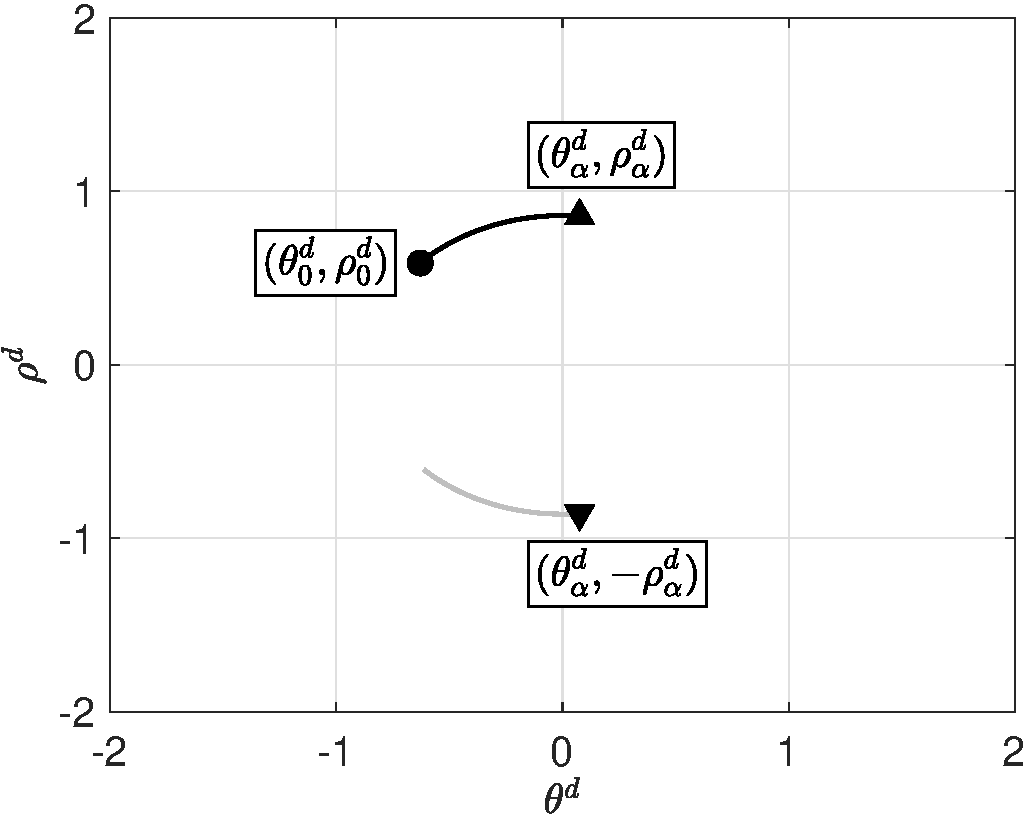
\includegraphics[width=0.48\textwidth]{img/stHMC_angle_illustration_rejected.pdf} ~~~
    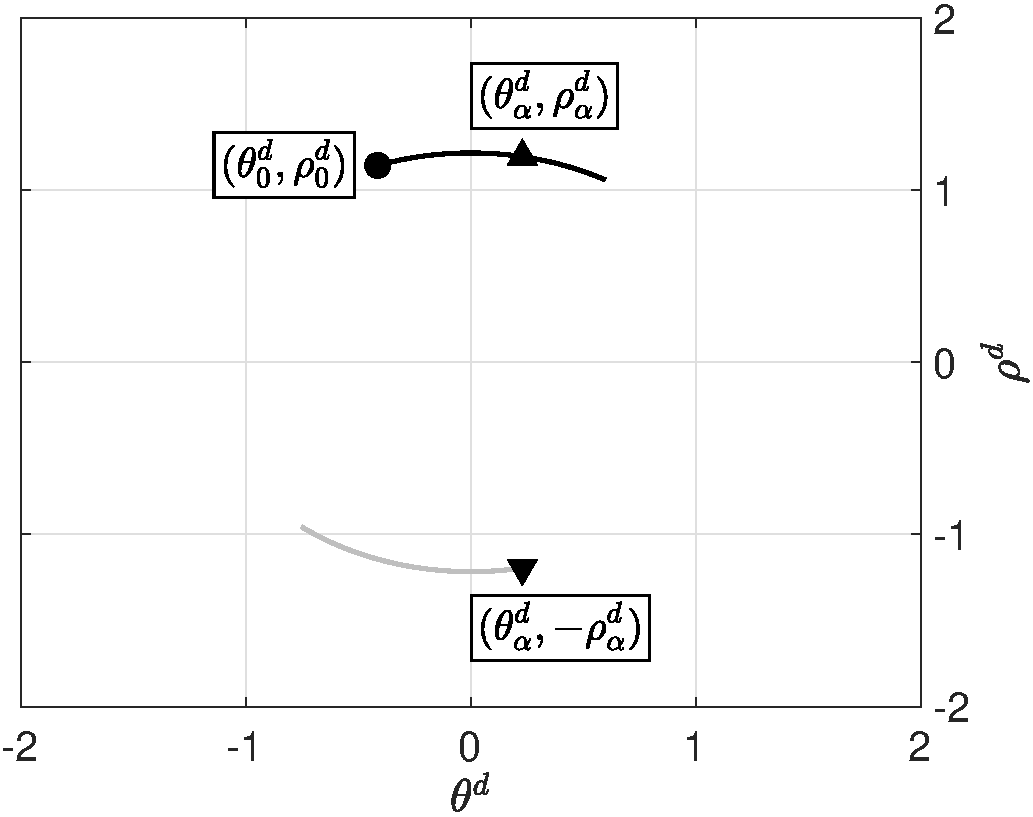
\includegraphics[width=0.48\textwidth]{img/stHMC_angle_illustration_accepted.pdf} 
        
    \caption{\it {\bfseries Self-Tuning Path Lengths for Exact HMC.} This figure plots forward and backward trajectories of the GIST sampler using \eqref{eq:ct_angle} in the phase space of the least constrained coordinate of the $d$-dimensional Gaussian measure with covariance matrix given in \eqref{eq:sigma_diag} with $d=10^3$.    The left panel illustrates a rejected proposal (due to $\alpha>\tau_2$) and the right panel illustrates an accepted proposal.}
    \label{fig:stHMC_illustration}
\end{figure}


\section{Path length sampling to avoid U-turns} \label{sec:step-distro} \label{sec:u-turn-avoiding}

We now turn to an extended example of a novel U-turn avoiding sampler based on Gibbs self tuning.  We will focus on locally adapting the number of steps.  Thus for each HMC step, the self-tuned HMC algorithm will generate the number of steps probabilistically according to a distribution $p(L \mid \theta, \rho, \epsilon, \Sigma)$.  We consider several such distributions based on the no U-turn condition in the next section and evaluate them in the following sections.

\newcommand{\pos}[2]{#1^{(#2)}}
\begin{figure}[t]
\small
\begin{flushleft}
$\textbf{GIST}(\theta, \rho, \epsilon, \Sigma)$
\vspace*{2pt}
\hrule
\vspace*{2pt}
\begin{tabular}{ll}
$\theta \in \mathbb{R}^d$ & initial position
\\[2pt]
$\rho \in \mathbb{R}^d$ & initial momentum (unused---discarded in Gibbs update)
\\[2pt]
$\epsilon \in (0, \infty)$ & step size
\\[2pt]
$\Sigma \in \mathbb{R}^{d \times d}$ & symmetric, positive definite mass matrix
\\[2pt]
$p(\theta)$ & target density (log density evaluation \& gradient)
\\[2pt]
$p(L \mid \theta, \rho, \epsilon, \Sigma)$ & conditional steps distribution (sampler \& log density evaluation)
\end{tabular}
\vspace*{4pt}
\hrule
\vspace*{6pt}
{\footnotesize (INITIALIZE)} \\[2pt]
$\pos{\theta}{0} = \theta$
\\[10pt]
{\footnotesize (GIBBS)} \\[2pt]
$\pos{\rho}{0} \sim \textrm{normal}(0, \Sigma)$ \hfill (Gibbs sample momentum)
\\[4pt]
$L \sim p(L \mid \pos{\theta}{0}\!,\, \pos{\rho}{0}\!,\, \epsilon, \Sigma)$ \hfill (Gibbs sample number of steps)
\\[10pt]
{\footnotesize (METROPOLIS-WITHIN-GIBBS)} \\[2pt]
for $\ell$ from $0$ to $L - 1$ (inclusive):  \hfill ($L$ leapfrog steps)
\\[-6pt]
\null \qquad $\pos{\rho}{\ell + 1/2} = \pos{\rho}{\ell} + \frac{\epsilon}{2} \cdot \nabla \log p(\pos{\theta}{\ell})$ \hfill (half step momentum)
\\[-6pt]
\null \qquad $\pos{\theta}{\ell + 1} = \pos{\theta}{\ell} + \epsilon \cdot \Sigma^{-1} \cdot \pos{\rho}{\ell + 1/2}$ \hfill (full step position)
\\[-6pt]
\null \qquad $\pos{\rho}{\ell + 1} = \pos{\rho}{\ell + 1/2} + \frac{\epsilon}{2} \cdot \nabla \log p(\pos{\theta}{\ell + 1})$ \hfill (half step momentum)
\\[6pt]
$\theta^*, \rho^* = \pos{\theta}{L}, -\pos{\rho}{L}$  \hfill (proposal flips momentum)
\\[4pt]
$u \sim \textrm{uniform}([0, 1])$ \hfill (sample acceptance probability)
\\[4pt]
if
$u < \frac{\displaystyle p(\theta^*\!\!,\, \rho^*\!\!,\,  L \mid \epsilon, \Sigma)}
         {\displaystyle p(\pos{\theta}{0}\!,\, \pos{\rho}{0}\!,\, L \mid \epsilon, \Sigma)}$
\hfill (Metropolis accept condition)
\\
\null \quad return $\theta^*\!\!,\, \rho^*\!\!,\, L$ \hfill (accept)
\\[4pt]
else
\\[-12pt]
\null \quad return $\null \quad \pos{\theta}{0}\!,\, \pos{\rho}{0}\!,\, L$ \hfill (reject)
\vspace*{2pt}
\hrule
\caption{\it {\bfseries GIST sampling for path-length self-tuning}.  The GIST sampler for path-length self-tuning differs from standard HMC in sampling the number of steps each iteration and then adjusting the acceptance probability to ensure detailed balance.  Note, the Gibbs steps for refreshment of both momentum and number of steps are exact draws from the corresponding conditional distributions.
}
\label{fig:self-tuning-hmc}
\end{flushleft}
\end{figure}

Figure~\ref{fig:self-tuning-hmc} provides pseudocode for a general algorithm adapting the number of leapfrog steps.  The ratio of the proposal joint density to the staring point joint density can be factored as
\[
\frac{\displaystyle p\!\left(\theta^*, \rho^*,  L^* \mid \epsilon, \Sigma\right)}
         {\displaystyle p\!\left(\pos{\theta}{0}, \pos{\rho}{0}, L^* \mid \epsilon, \Sigma\right)}
\ = \ 
\frac{\displaystyle p\!\left(\theta^*\right)}
     {\displaystyle p\!\left(\pos{\theta}{0}\right)}
\cdot 
\frac{\displaystyle p\!\left(\rho^* \mid \Sigma\right)}
     {\displaystyle p\!\left(\pos{\rho}{0} \mid \Sigma\right)}
\cdot
\frac{\displaystyle p\!\left(L^* \mid \theta^*, \rho^*, \epsilon, \Sigma\right)}
     {\displaystyle p\!\left(L^* \mid \pos{\theta}{0}, \pos{\rho}{0}, \epsilon, \Sigma\right)},
\]
where $p(\theta) = p(\theta \mid y)$ is the target probability density function, $p(\rho \mid \Sigma) = \textrm{normal}(0, \Sigma)$ is the momentum probability density function, and $p(L \mid \theta, \rho, \epsilon, \Sigma)$ is the conditional step size probability mass function.


\subsection{Step distributions avoiding U-turns} 

\begin{figure}[t]
\usetikzlibrary{arrows.meta, angles, quotes, calc}
\begin{center}
\begin{tikzpicture}[>=Stealth]
  % Define points along the arc
  \coordinate (A) at (0,0);
  \coordinate (B) at (2,2);
  \coordinate (C) at (4,1);
  \coordinate (D) at (6,3); % Second to last point
  \coordinate (E) at (8,2); % Last point

  \node at (A) [below=0.125cm] {$\pos{\theta}{0}$};
  \node at (B) [above=0cm] {$\pos{\theta}{1}$};
  \node at (C) [below=0.125cm] {$\pos{\theta}{2}$};
  \node at (D) [above=0cm] {$\pos{\theta}{3}$};
  \node at (E) [below=0.125cm] {$\theta^*$};

  % Draw trajectory with arrows
  \draw[->] (A) -- (B);
  \draw[->] (B) -- (C);
  \draw[->] (C) -- (D);
  \draw[->,style=dashed] (D) -- (E);

  % Place solid circles at discretized positions
  \foreach \point in {A,B,C,D,E}
    \fill (\point) circle (2pt);

  % Dotted line from first to second to last point
  \draw[dotted] (A) -- (D);

  % Auxiliary point for angle calculation
  % This creates an invisible point extending the dotted line beyond 'D' for angle drawing
  \coordinate (F) at ($(A)!-1.2!(D)$); % Extend line beyond D for angle marking

  % Arc for angle indication
  \pic[draw, ->, "$\alpha$", angle eccentricity=1.5, angle radius=1cm] {angle = F--D--E};
\end{tikzpicture}
\end{center}
\caption{\it {\bfseries U-turn condition.}  A Hamiltonian trajectory of positions (not momenta) in two dimensions, consisting of three leapfrog steps plus a potential fourth step.  The dotted line connects the initial position $\pos{\theta}{0}$ to the current position $\pos{\theta}{3}$.  The dashed line connects the current position to the next potential position $\theta^*$ and runs in the direction of the current momentum $\pos{\rho}{3}$.  The trajectory is extended one step to $\theta^*$ if the next step moves away from the initial position, which requires the absolute value of the angle $\alpha$ between the dotted line and the dashed line to be greater than $90^\circ$, which arises when $(\pos{\theta}{3} - \pos{\theta}{0})^\top \cdot (\theta^* - \pos{\theta}{3}) > 0$, or equivalently, when $(\pos{\theta}{3} - \pos{\theta}{0}) \cdot \pos{\rho}{3} > 0.$}
    \label{fig:u-turn-condition}
\end{figure}

To make our sampler concrete, a specific distribution over the number of steps must be defined.  We evaluate a few related choices, all of which are motivated by the observation driving the No U-Turn Sampler (NUTS) \cite{HoGe2014}, which is that it's wasteful to evaluate the Hamiltonian dynamics beyond the point at which the trajectory has made a U-turn and is heading back toward the starting position.  Figure~\ref{fig:u-turn-condition} illustrates the U-turn condition, which is made precise in Equation~(\ref{eq:uturn-cond}).  

Let $\textrm{U}(\theta, \rho, \epsilon, \Sigma)$ be the maximum number of leapfrog steps that can be taken before a U-turn, starting from $(\theta, \rho)$ and using step size $\epsilon$ and mass matrix $\Sigma$.  The point just before a U-turn can be defined for the discrete steps of the leapfrog integrator by
\begin{equation}\label{eq:uturn-cond}
\textrm{U}\!\left(\pos{\theta}{0}\!,\, \pos{\rho}{0}\!,\, \epsilon, \Sigma\right)
= \textrm{arg min}_{n \in \mathbb{N}} \ \left(\pos{\theta}{n} - \pos{\theta}{0}\right)^\top \cdot \pos{\rho}{n} < 0,
\end{equation}
where $\pos{\theta}{n}\!, \pos{\rho}{n}$ is the location in phase space after $n$ leapfrog steps from $\pos{\theta}{0}\!, \pos{\rho}{0}$ with step size $\epsilon$ and positive-definite mass matrix $\Sigma.$  

\begin{figure}[t]
    \centering
\begin{tikzpicture}[node distance=1.5cm and 0.75cm]
    % Top row nodes
    \node[circle,draw,minimum size=1cm] (LM) {\footnotesize $L{-}N$};
    \node[minimum size=1cm,right of=LM] (dots1) {$\cdots$};
    \node[circle,draw,minimum size=1cm,right of=dots1] (0) {$0$};
    \node[minimum size=1cm,right of=0] (dots2) {$\cdots$};
    \node[circle,draw,minimum size=1cm,right of=dots2] (L) {$L$};
    \node[minimum size=1cm,right of=L] (dots3) {$\cdots$};
    \node[circle,draw,minimum size=1cm,right of=dots3] (N) {$M$};
    
    % 2nd row nodes
    \node[below = 0.05cm of LM] (n_a1) {$\strut$};
    \node[below = 0.05cm of 0] (theta_rho) {$\strut (\theta, \rho)$};
    \node[below = 0.05cm of L] (theta_rho_star) {$\strut (\theta^*, \rho^*)$};
    \node[below = 0.05cm of N] (n_a2) {$\strut$};

    
    % 3rd row arrow
    \node[below = -0.25cm of n_a1] (n_a3) {$\strut$};
    \node[below = -0.25cm of theta_rho] (start_arrow2) {$\strut$};
    \node[below = -0.25cm of theta_rho_star] (n_a4) {$\strut$};
    \node[below = -0.25cm  of n_a2] (end_arrow2) {$\strut$};
    \draw[->, line width=1pt] (start_arrow2) -- (end_arrow2) node[midway, below] {$M = U(\theta, \rho, \epsilon, \Sigma)$};
    
    % 4th row arrow
    \node[below = 0.05cm of n_a4] (start_arrow1) {$\strut$};
    \node[below = 0.05cm of n_a3] (end_arrow1) {$\strut$};
    \draw[->, line width=1pt] (start_arrow1) -- (end_arrow1) node[midway, below] {$N = U(\theta^*, \rho^*, \epsilon, \Sigma)$};
\end{tikzpicture}
    \caption{\it {\bfseries Self-tuned steps proposal.} Starting from the initial position and momentum $(\theta, \rho)$, the algorithm makes $M$ forward leapfrog steps until a U-turn.  It then Gibbs samples a number of steps $L$ between 0 and $M$ for which the leapfrog integrator produces the proposal $(\theta^*, \rho^*)$.  Then $N$ backward leapfrog steps are taken until a U-turn.
    If $L - N > 0,$ the proposal is rejected.  The algorithm takes $M + N - L$ unique leapfrog steps.}
    \label{fig:adaptive-u-turns}
\end{figure}  
Figure~\ref{fig:adaptive-u-turns} shows a single step of the algorithm.  The number of steps is sampled conditionally based on the number of steps possible before a U-turn.  To preserve detailed balance, the trajectory from the selected point backward in time is evaluated until it makes a U-turn and the probability of selecting the initial state (i.e., the same number of steps) is used to balance the selection.  This requires sampling zero or more steps backward in time before the initial position.

\subsection{Conditional distribution of steps} 

In this section, we consider a few closely related approaches to generating the number of steps given the number of steps to a U-turn.  

\subsubsection{Steps generated uniformly}

The most obvious choice for a conditional distribution over the number of steps is uniform between 1 and the number of steps before a U-turn,
\begin{equation}
p(L \mid \theta, \rho, \epsilon, \Sigma)
= \textrm{uniform}\!\left(L \mid 1, \, \textrm{U}(\theta, \rho, \epsilon, \Sigma)\right),
\end{equation}
where the bounds are read inclusively.

\subsubsection{Steps generated uniformly from later states}

One of the techniques NUTS uses to take such long jumps on average is to bias the selection of a candidate toward the end of the Hamiltonian trajectory \cite{HoGe2014}.  To create a simple approximation to this, the uniform distribution can be restricted to the latter part of the trajectory by changing the lower bound from 1 to something greater.  Any number between 0 and $M = \textrm{U}(\theta, \rho, \epsilon, \Sigma)$ is valid as a lower bound.  The choice of 1 corresponds to the uniform distribution of the previous section.  We will also evaluate lower bounds of $\lfloor \frac{1}{2} \cdot M \rfloor$ and $\lfloor \frac{3}{4} \cdot M \rfloor$, where $\lfloor x \rfloor$ is the floor of $x$, which is largest integer less than or equal to $x$.  With smaller intervals, the proposed trajectory lengths will be longer, but the reversibility balance condition will reduce the acceptance probability.

\subsubsection{Binomial step generation}

Non-uniform distributions may also be used.  For example, a binomial distribution for the number of steps could be defined for a fixed $\psi \in (0, 1)$ as 
\begin{equation}
    p(L \mid \theta, \rho, \epsilon, \Sigma)
    = \textrm{binomial}\!\left(L \mid \psi, \, \textrm{U}(\theta, \rho, \epsilon, \Sigma)\right).
\end{equation}
The expected value of $L$ starting from $(\theta, \rho)$ is thus $\psi \cdot \textrm{U}(\theta, \rho, \epsilon, \Sigma).$  We evaluated the binomial method and it winded up generating proposals that were too concentrated and thus hard to balance and accept, so we do not include results here.  We did not evaluate a more dispersed beta-binomial distribution due to the cost of the beta and gamma functions required for normalization.



\section{Empirical evaluation}\label{sec:experiments}

In this section, we evaluate the performance of our various proposals for step size adaptation and compare their performance to the state-of-the-art No U-Turn Sampler as coded in Stan \cite{HoGe2014,betancourt2017conceptual}.  


\subsection{Models evaluated}

The models considered are multivariate standard normal, ill-conditioned multivariate normal, correlated multivariate normal, eight schools meta-analysis, item-response theory 2 parameter logistic model, mixed effects Poisson regression, normal mixture, hidden Markov model, one-compartment pharmacokinetic / pharmacodynamic model (PK/PD), Lotka-Volterra population dynamics, autoregressive time series (AR), autoregressive moving average time series (ARMA), and generalized autoregressive conditional heteroskedasticity time series (GARCH).  All but the normal models are drawn from the \texttt{posteriordb} package \cite{posteriordb2023}, but reparameterized according to Stan best practices so that NUTS can sample them.

\begin{figure}[t]
    \centering
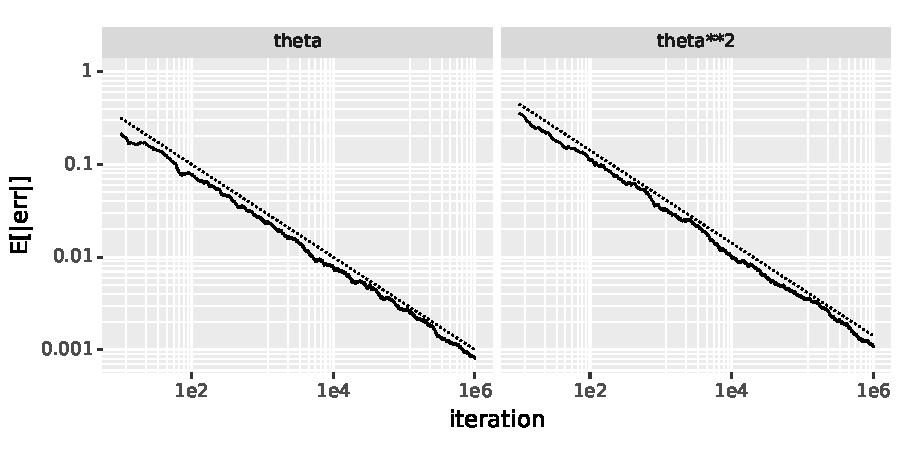
\includegraphics[width=0.48\textwidth]{img/results/uniform/learning_curve_iid.pdf}
\hfill
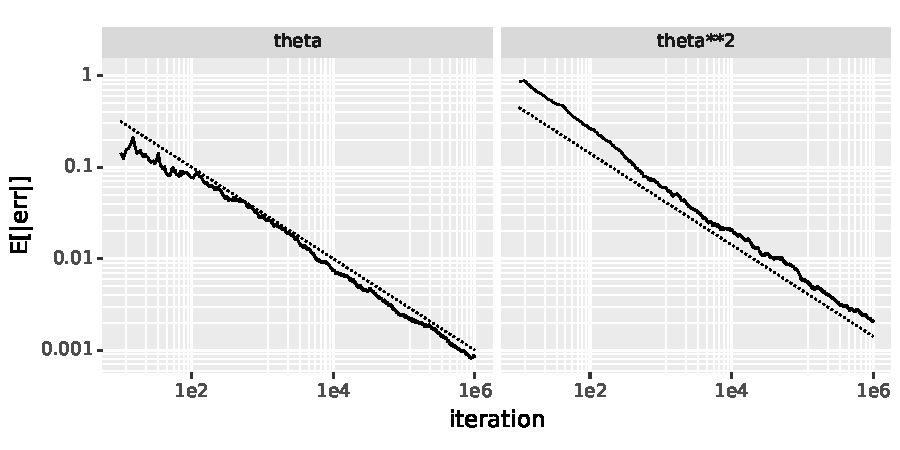
\includegraphics[width=0.48\textwidth]{img/results/uniform/learning_curve_uniform_full_100D.pdf}
\vspace*{-9pt}
\caption{\it {\bfseries Learning curve validation.} The absolute error in parameter and parameter squared estimates for i.i.d. draws (left) and the uniform self-tuning algorithm (right).  In each plot, the left half shows error for parameter estimates and the right half shows error for squared parameter estimates (averaged over the 100 identical dimensions).  For reference, the dotted line is the standard error derived from independent draws, which at iteration $n$ is $1 / \sqrt{n}$ for parameter estimates and $\sqrt{2}\, / \sqrt{n}$ for squared parameter estimates.}
\label{fig:learning-curve}
\end{figure}

\subsection{Learning curve}

As a simple validation that the sampler is targeting the correct distribution, Figure~\ref{fig:learning-curve} plots a learning curve (expected absolute error) versus iteration for the uniform sampler with the full path for the eight schools model. The plot shows that error decreases as expected at a rate of $1 / \sqrt{n}$ and the efficiency is greater than that of independent draws for the parameters and slightly worse for the parameters squared in this simple case.


\subsection{Effect of step size and path fraction}

\begin{figure}[t]
\begin{center}
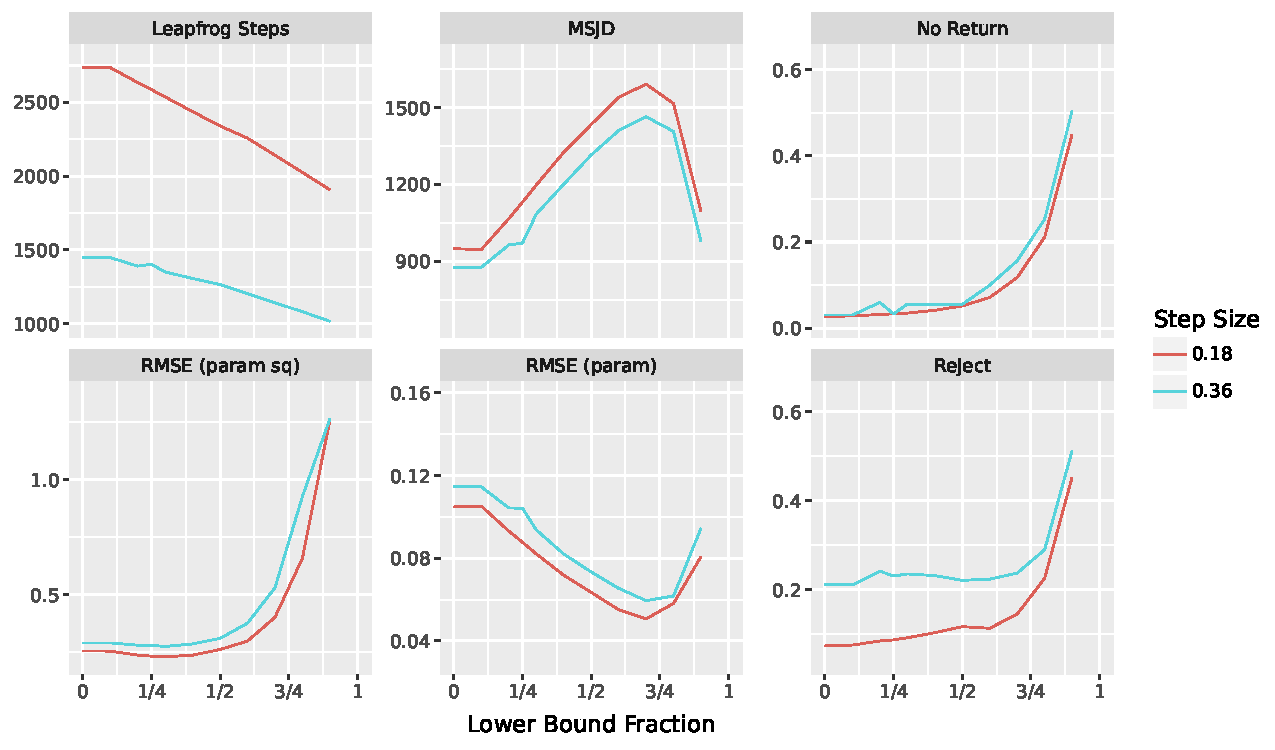
\includegraphics[width=0.8\textwidth]{img/results/uniform/uniform_prob_steps_plot.pdf}
\end{center}
\caption{\it {\bfseries Performance versus step size and lower bound fraction}.  The plots represent averages (over 200 repetitions) of results for 100 iterations of uniform self-tuning HMC starting from a draw from the 500-dimensional standard normal target distribution.  The $x$-axis represents the fraction of the number of steps to a U-turn to use as the lower bound in uniformly drawing a number of leapfrog steps.  Line color indicates step sizes 0.36 (blue) and 0.18 (red).  The titles of the subplots describe the values on the $y$-axis.  The label "No Return" (top right) is for the fraction of non-reversible proposals due to a U-turn before returning to the starting point, and the proportion of rejections (lower right) includes those due to non-reversibility.}\label{fig:step-lb-uniform}
\end{figure}

In Figure~\ref{fig:step-lb-uniform}, the performance of the uniform self-tuning sampler is shown for two step sizes, 0.36 (blue lines) and 0.18 (red lines), across a range of lower bound fractions ($x$ axis) for uniform sampling.  The step size 0.36 is what NUTS adapted for an 80\% average Metropolis acceptance probability (Stan's default); 0.18 is the step size for roughly 95\% Metropolis acceptance.  Halving the step size roughly doubles the number of leapfrog steps taken, as shown in the upper left of the plot.  The remaining plots show that performance is better with a smaller step size.  

Mean square jump distance (MSJD) is also shown in Figure~\ref{fig:step-lb-uniform}; it is defined for $M$ steps of sampling by
\begin{equation}
\textrm{MSJD}
= \frac{1}{M} \sum_{m = 1}^M \left|\left|\pos{\theta}{m+1} - \pos{\theta}{m}\right|\right|_2^2.
\end{equation}
The MSJD is a reasonable estimate of the expected squared jump distance, 
\begin{equation}
\textrm{ESJD}
= \mathbb{E}\!\left[\left|\left|\pos{\theta}{t+1} - \pos{\theta}{t}\right|\right|^2_2\right].
\end{equation}
As the path fraction goes up, the MSJD goes up until the no-return rejection rate overtakes it and it begins to decrease. 

The rejection rate is broken down into total rejection rate, and then the number of rejections due to not being able to return to the origin before hitting a U-turn (see Figure~\ref{fig:adaptive-u-turns}).  Smaller step sizes do a better job at preserving the Hamiltonian and thus have lower rejection rates.  

Root mean square error (RMSE) is defined by
\begin{equation}
\textrm{RMSE} = \sqrt{\frac{1}{M} \sum_{m=1}^M \left|\left|\pos{\theta}{m} - \theta\right|\right|_2^2},
\end{equation}
where $\theta$ is the value of the parameter and the $\theta^{(m)}$ are MCMC draws.  If the draws were independent, the expected RMSE for parameters is 0.1 (the standard deviation, 1, divided by the square root of the number of i.i.d. draws, $\sqrt{100}$).  The expected RMSE for parameters squared is $\sqrt{2} / 10$ because standard normal variates squared follow a chi-squared distribution with 1 degree of freedom, the standard deviation of which is $\sqrt{2}$.  The RMSE for parameters is below that of independent draws, going down to roughly half at lower bound fraction 0.6.  Not surprisingly, because MSJD tracks inverse lag-one autocorrelation, the best RMSE for parameters is achieved where the MSJD is maximized.  The RMSE for parameters squared is mazimized at around a 0.35 lower-bound fraction, though values are very close between 0 and 1/2.  With a single lower bound fraction, a trade off must be made, as it must be for HMC and NUTS.  Here a fraction of 0.6 appears reasonable.  The RMSE is lower for the smaller step sizes, but doubling the number of iterations with the larger step size would reduce expected RMSE by a factor of $1 / \sqrt{2}$ (about 70\%).


\subsection{Evaluations for multiple models}

\begin{figure}[th]
    \centering
    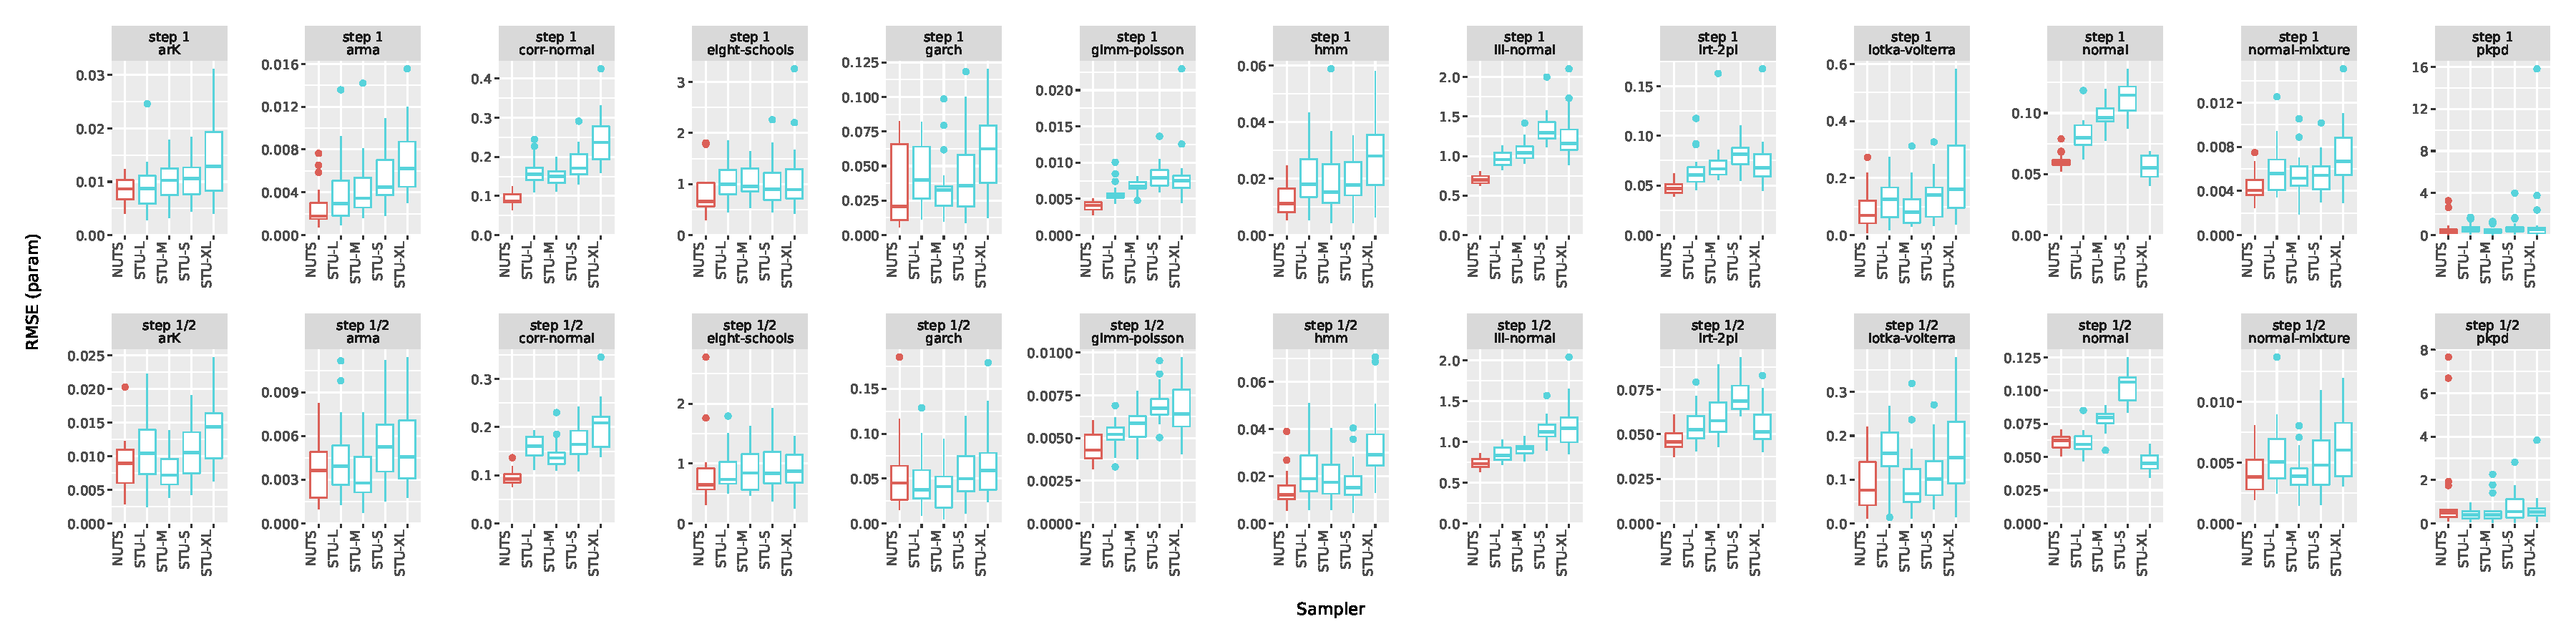
\includegraphics[width=0.95\textwidth]{img/results/uniform/vs_nuts_RMSE_param.pdf}
    %
    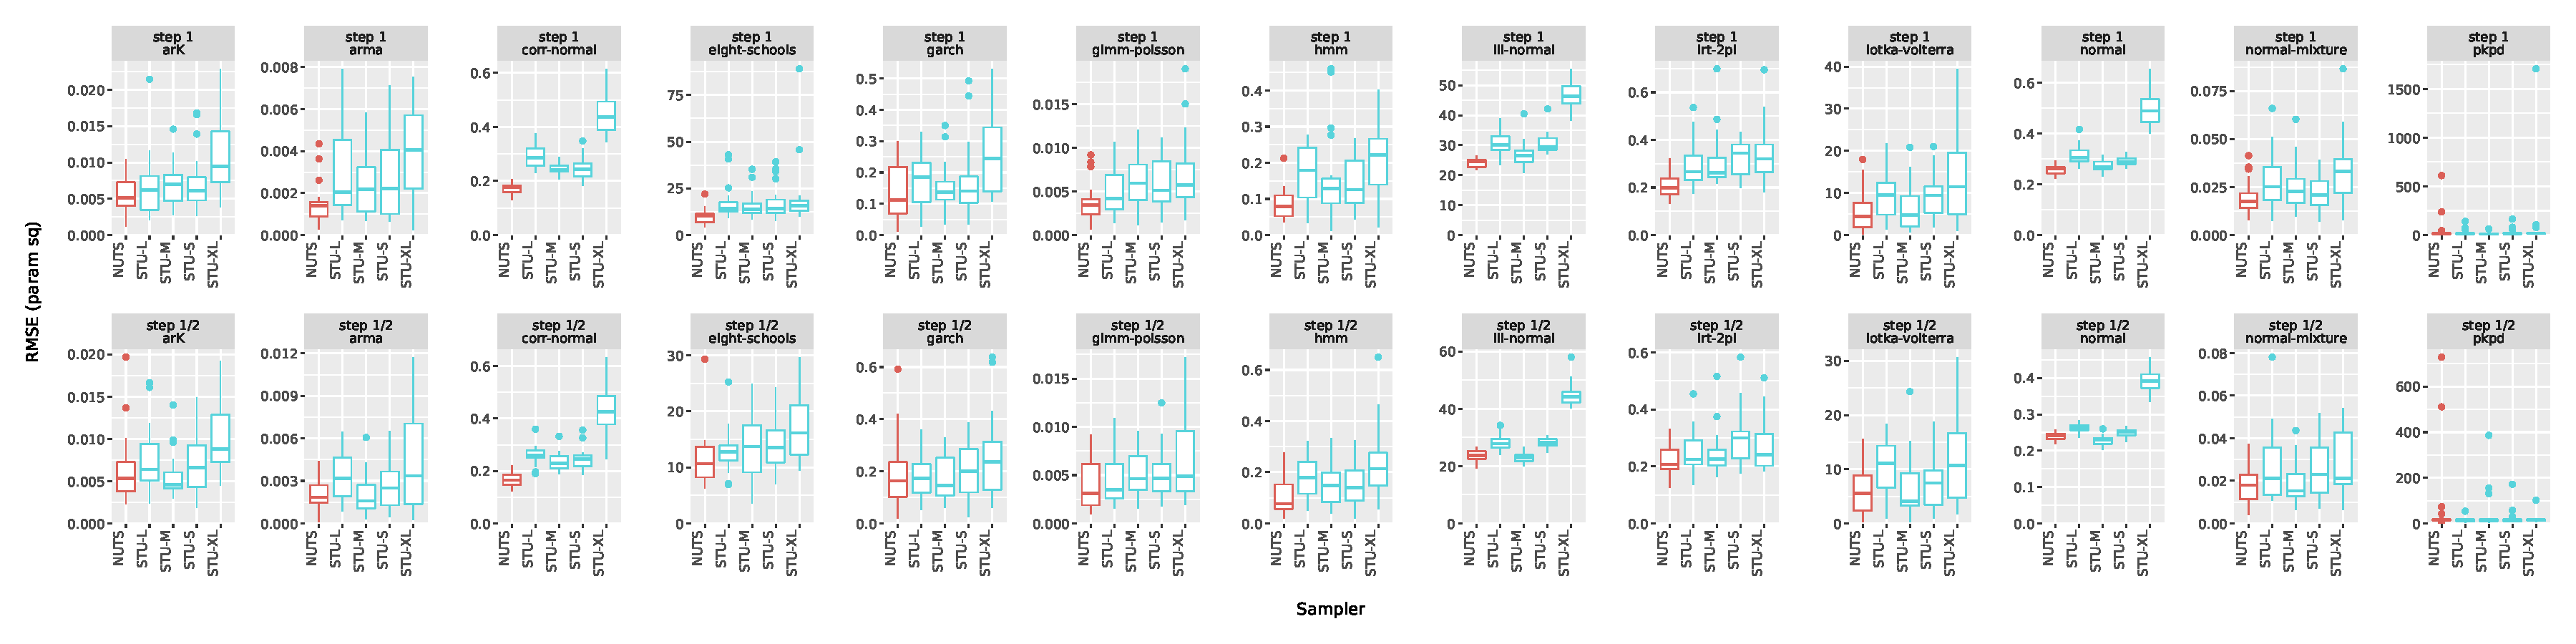
\includegraphics[width=0.95\textwidth]{img/results/uniform/vs_nuts_RMSE_param_sq.pdf}
    %
    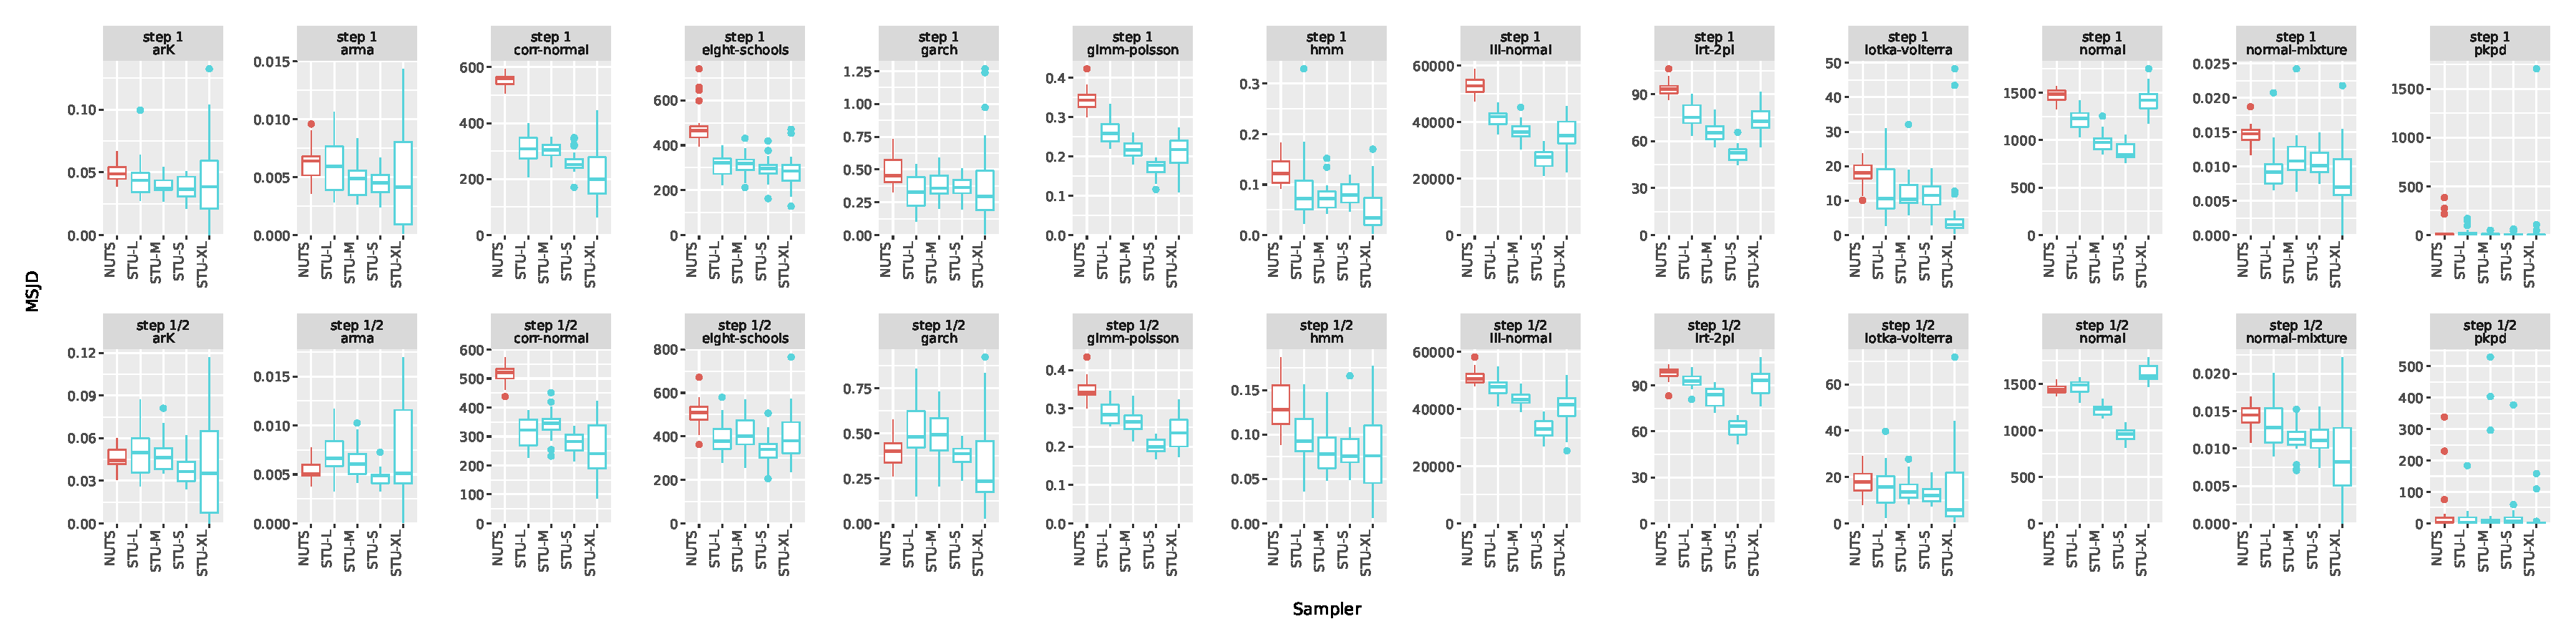
\includegraphics[width=0.95\textwidth]{img/results/uniform/vs_nuts_MSJD.pdf}
    %
    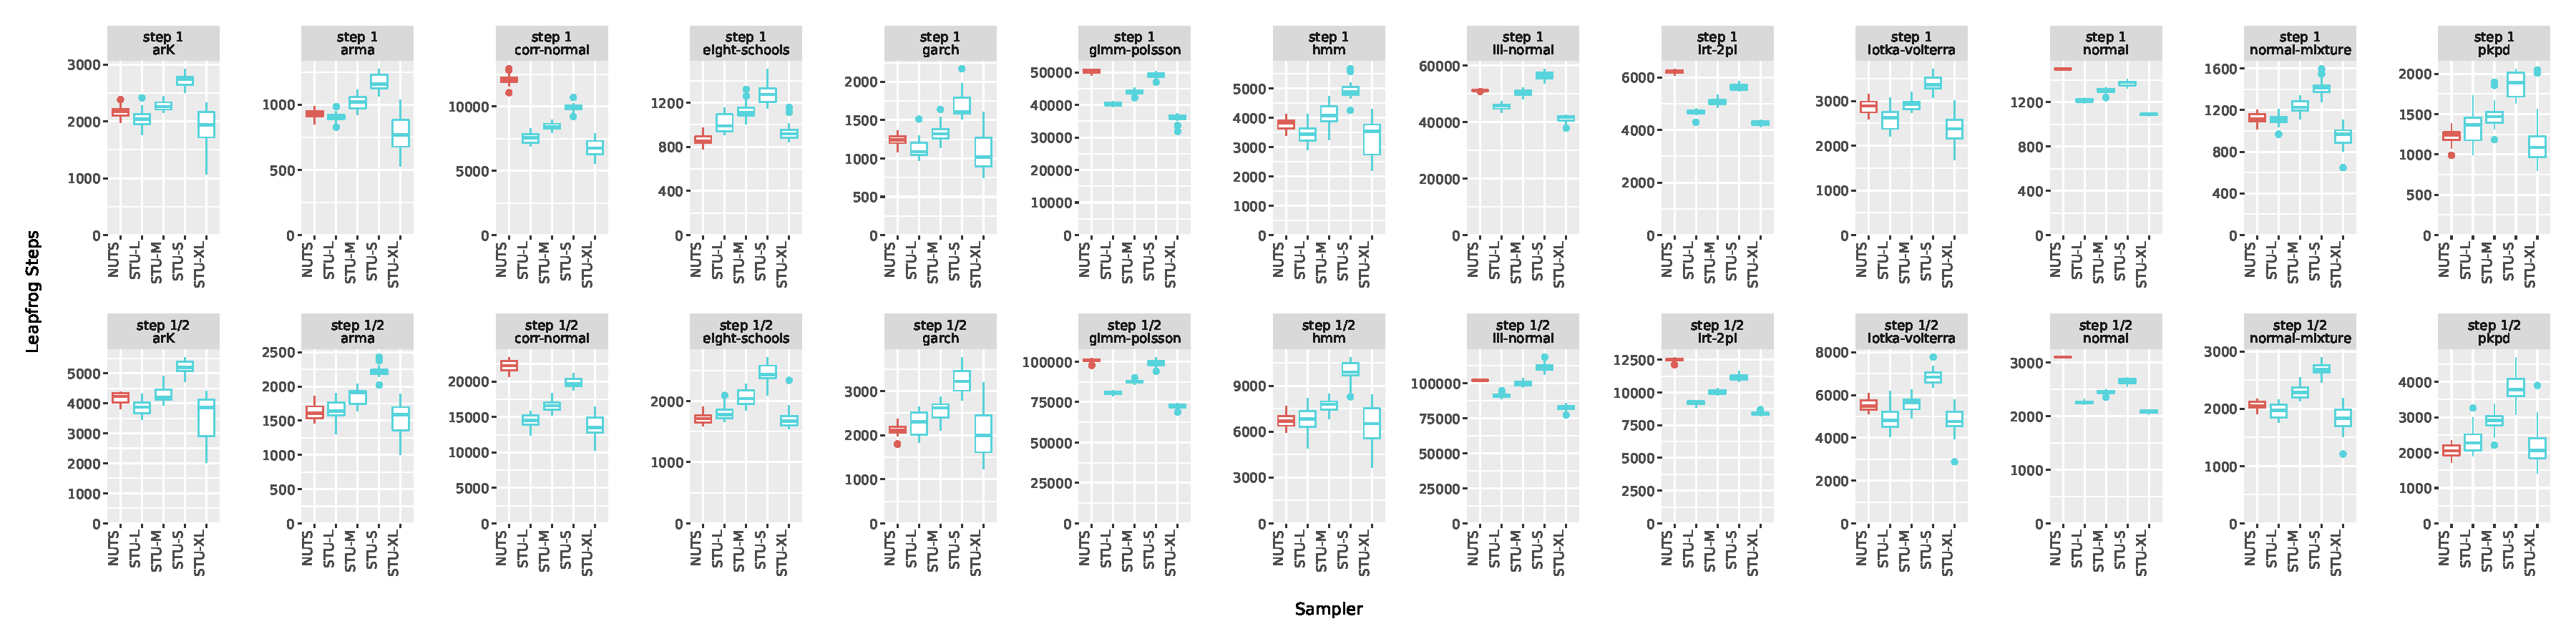
\includegraphics[width=0.95\textwidth]{img/results/uniform/vs_nuts_Leapfrog_Steps.pdf}
    \caption{\it {\bfseries Empirical Evaluations vs.~NUTS}. From top to bottom: root mean square error of parameters, root mean square error of parameters squared (lower is better), mean square jump distances (higher is better), and number of leapfrog steps (smaller is more efficient).  Each column is for a different model and the rows are for runs at NUTS default adapted step size (targeting 0.8 average Metropolis acceptance) and half of that rate (which targets approximately a 0.95 Metropolis acceptance, which increases stability of the leapfrog integrator).  The red result is NUTS and the blue results are for the self-tuning uniform sampler over intervals with 0.0 (S), 0.3 (M), 0.5 (L), and 0.7 (XL) path fraction.}
    \label{fig:empirical-evals}
\end{figure}
%
We run all of our reference models for 10,000 warmup and 40,000 iterations of NUTS using Stan's defaults and use the sampling draws to define reference means for parameters and parameters squared.  The results for the uniform sampler are shown in Figure~\ref{fig:empirical-evals}.  There are four plots, which show RMSE for parameters, RMSE for squared parameters, MSJD, and leapfrog steps.  

We evaluate NUTS (in red) and three settings of uniform sampling, S(hort), which uses $\textrm{uniform}(1, L)$ sampling, where $L$ is the number of steps to a U-turn, M(edium), which uses $\textrm{uniform}(\lfloor 0.3 \cdot L \rfloor, L)$, and L(ong), which uses $\textrm{uniform}(\lfloor 0.5 \cdot L \rfloor, L),$ and XL (extra long), which uses $\textrm{uniform}(\lfloor 0.7 \cdot L, L)$ sampling.  Two step sizes are considered, (1) the step size adapted by NUTS with its default acceptance target (80\%), and (1/2), which is half of that step size, which is approximately what NUTS would adapt for a target of 95\% step size, which is recommended for the numerical stability of the leapfrog integrator in more difficult problems.

Starting with leapfrog steps (the bottom plot), it is clear that the shorter expected paths require more steps for self-tuning HMC, because they are likely to have to go further past the origin backward in time before hitting a U-turn.  There is never more than a factor of two difference among systems in terms of leapfrog steps.  The steps required for NUTS and ST-HMC are similar; for some models, ST-HMC requires fewer steps than NUTS and for others it requires more steps. For the three normal cases, ST-HMC requires fewer steps for the standard normal and correlated normal, but about the same number for the ill-conditioned normal.

Smaller step sizes lead to roughly twice as many leapfrog steps, but not quite that in complicated models (or models that run up against the 1024 maximum step limit imposed on both NUTS and ST-HMC).

The second plot from the bottom shows the MSJD for all samplers, which is inversely related to autocorrelation at lag 1.  The clear trend is that larger steps lead to lower error, but this is not always borne out.  For instance, in the standard normal, the ST-HMC sampler takes longer steps and improves the estimate of parameters, but NUTS has lower error estimating parameters squared.

The first two plots show RMSE for parameters and parameters squared.  All plots have a $y$-axis starting at 0 so that relative performance may be assessed visually.  Many of the more complicated models are neck and neck in RMSE for parameters and parameters squared, with NUTS consistently slightly outperforming ST-HMC.  

In conclusion, NUTS slightly outperforms ST-HMC overall.  This is highly encouraging in that this is a relatively simple first attempt at self-tuned HMC, whereas NUTS is represented by Stan's current implementation, which has been implemented robustly and improved considerably over the first NUTS paper (and first version in Stan) \cite{betancourt2017conceptual,HoGe2014}.


\subsection{Open-source code and reproduciblity}

The results and plots can be reproduced from our code distribution, which is available from GitHub under a permissive open-source license.\footnote{The code is distributed under the MIT License at \url{https://github.com/bob-carpenter/adaptive-hmc}.}

\section{Other Related Prior work}

The GIST sampler may be viewed as a dynamic version of the empirical HMC sampler \cite{wu2018faster}. This empirical HMC sampler learns an empirical distribution of the underlying path lengths to U-turns during a warmup phase and then fixes this empirical distribution, which is then used to sample path lengths at each step during sampling. Like randomized HMC in Section~\ref{ex:exact_rHMC}, the empirical HMC sampler is an instance of the GIST sampler where the conditional distribution of path lengths does not depend on the current position and/or momentum.

Both NUTS and the Apogee-to-Apogee Path Sampler reviewed in Section ~\ref{sec:pathlength} can be formulated within the dynamic HMC framework introduced in \cite{durmus2023convergence}. Dynamic HMC can be viewed as an instance of a generalized Hit-and-Run sampler in the sense of \cite{Diaconis2007HitandRun}. On the other hand, as discussed in Section~\ref{sec:sthmc}, the GIST sampler is a Gibbs sampler (with a Metropolis-within-Gibbs step) aimed at the enlarged target measure \eqref{eq:enlarged_target}.  A key benefit of incorporating a Metropolis-within-Gibbs step in GIST is that it relaxes the restrictive symmetry conditions required for correctness of dynamic HMC in practice, and hence, offers significant flexibility to adapt other algorithm tuning parameters.

The autoMALA sampler introduced a self-tuning version of the Metropolis-adjusted Langevin (MALA) sampler \cite{kleppe2016adaptive,biron2024automala}.  It uses a forward and reverse non-deterministic scheme to choose adaptation parameters in a way that satisfies detailed balance. MALA is equivalent to one-step Hamiltonian Monte Carlo, but is simpler in not needing to evolve momentum.  The GIST sampler can be viewed as a probabilistic generalization of the autoMALA adaptation selection criteria.

For step size and mass matrix tuning, two approaches have been popular in practice. In the first, an adaptation phase is used to estimate algorithm tuning parameters. These tuning parameters are then fixed so that the resulting chain is Markovian. This is the strategy used by NUTS for step size and mass matrix adaptation for HMC \cite{HoGe2014}. In the second approach, the adaptation phase is never turned off, but the amount of adaptation is decreased so that asymptotically the results are valid.  This is the strategy used by delayed rejection Metropolis (DRAM) \cite{haario2006dram}.

Another approach for step size adaptivity is the recently introduced delayed rejection HMC sampler of \cite{modi2023delayed}.  The delayed rejection algorithm \cite{mira2001metropolis,green2001delayed} is a generalization of Metropolis-Hastings to a sequence of proposal moves.  This proposal sequence can be tuned to start with larger scale moves and then scaled down for subsequent proposals \cite{haario2006dram}. In the same vein, the delayed rejection HMC sampler automatically tries smaller step sizes if proposals with larger step sizes are rejected, allowing it to sample from target densities with varying scale. Like other delayed rejection methods, it generates ``ghost points'' using reversed proposals, which are then used as part of the acceptance probability to ensure detailed balance \cite{green2001delayed}.


\subsection*{Acknowledgements}

We would like to thank Edward Roualdes, Tore Kleppe, Andreas Eberle, Sam Livingstone, and Chirag Modi for feedback on the Gibbs self-tuning idea.

N.~Bou-Rabee has been partially supported by NSF Grant No.~DMS-2111224.


\printbibliography

\appendix

\section{Proof of correctness}\label{app:proof_of_correctness}

The correctness of the GIST sampler given in Figure~\ref{fig:general-self-tuning-step}  follows from the observation that the GIST sampler is a Gibbs sampler which interleaves Gibbs resampling of the velocity variable $\rho$ and tuning parameter $\alpha$ with a Metropolis-within-Gibbs step that uses a proposal given by a  measure-preserving involution. In fact, this idea is also the essence of the standard HMC sampler, and the GIST sampler is a natural extension of this idea to the selection of tuning parameters as well.

The proof of correctness relies on the following general lemma. This lemma is not new; see, e.g.,  special case 2 of Theorem 2 in \cite{Tierney1998}.  However, a complete proof is given for the reader's convenience.

\begin{lemma} \label{lem:DeterministicMetropolization} 
Suppose that $(\mathbb{S}, \mathcal{F}, \lambda)$ is a measure space, $\nu$ is a probability measure with strictly positive density $ \gamma$ with respect to $\lambda$, and $F: \mathbb{S}\to \mathbb{S}$ is a measurable involution which preserves $\lambda$. Given a state $Z \in \mathbb{S}$, define a Markov transition kernel by the following procedure:
\begin{itemize}
    \item Draw $\mathcal{U} \sim \operatorname{uniform}([0,1])$.
    \item Set $Z' = F(Z)$ if  $\mathcal{U} \le \min\left(1, \frac{\gamma(F(Z))}{\gamma(Z)} \right)$ and $Z' = Z$ otherwise.
\end{itemize}
Then, this transition step is reversible with respect to $\nu$.
\end{lemma}


\begin{proof}[Proof of Lemma~\ref{lem:DeterministicMetropolization}]
Let $Z \sim \nu$.  The proof shows that \[
\prb(Z  \in A , Z' \in B) =  \prb(Z'  \in A , Z \in B) \;, 
\] 
for all measurable sets $A,B \in \mathcal{F}$.
Let $\beta(x,F(x)) = \min \left(1, \frac{\gamma(F(x))}{\gamma(x)} \right)$ for all $x \in \mathbb{S}$. For all $x \in \mathbb{S}$ and for any measureable set $A \in \mathcal{F}$, the  transition kernel associated to the transition step described in Lemma~\ref{lem:DeterministicMetropolization} is given by \[
p(x, A) = \beta(x,F(x)) \delta_{F(x)}(A) + (1 - \beta(x, F(x))) \delta_{x}(A) \;.
\] Hence,
\begin{align}
\prb( & Z  \in A , Z' \in B) = \int_A p(x,B) \nu(dx) \notag \\
&= \int_A \left[ \beta(x, F(x)) \mathds{1}_B(F(x)) + (1 - \beta(x,F(x))) \mathds{1}_B(x) \right] \nu(dx) \label{eq:metrodef} \\
&= \int_\mathbb{S} \left[ \beta(x, F(x)) \mathds{1}_B(F(x)) \mathds{1}_A(x) + (1 - \beta(x,F(x)))\mathds{1}_A(x)\mathds{1}_B(x) \right] \nu(dx) \;. \label{eq:metropolisexpansion}
\end{align}
The second term in \eqref{eq:metropolisexpansion} is already symmetric in the sets $A,B$ --- so we turn our attention to the first term. For this term, we use the elementary identity $a \min(1, \frac{b}{a}) = b \min(1, \frac{a}{b})$ valid for all $a, b \ne 0$, as follows  \begin{align}
\int_\mathbb{S} & \beta(x, F(x)) \mathds{1}_B(F(x)) \mathds{1}_A(x) \nu(dx)  \nonumber \\
&= \int_\mathbb{S} \beta(x, F(x)) \mathds{1}_B(F(x)) \mathds{1}_A(x) \gamma(x) \lambda(dx) \notag \\
&= \int_\mathbb{S} \mathds{1}_B(F(x)) \mathds{1}_A(x) \gamma(x) \min \left(1, \frac{\gamma(F(x))}{\gamma(x)} \right) \lambda (dx) \notag \\
&= \int_X \mathds{1}_B(F(x)) \mathds{1}_A(x) \gamma(F(x)) \min \left(1, \frac{\gamma(x)}{\gamma(F(x))} \right) \lambda (dx) \;. \notag 
\end{align}
But, since the map $F$ preserves $\lambda$ and is an involution we have, by change of variables under $F$,
\begin{align}
 \int_\mathbb{S} & \mathds{1}_B(F(x)) \mathds{1}_A(x) \gamma(F(x)) \min \left(1, \frac{\gamma(x)}{\gamma(F(x))} \right) \lambda (dx) \nonumber \\
& = \int_\mathbb{S} \mathds{1}_B(F(F(x))) \mathds{1}_A(F(x)) \gamma(F(F(x))) \min \left(1, \frac{\gamma(F(x))}{\gamma(F(F(x)))} \right) \lambda (dx) \nonumber  \\
&=\int_{\mathbb{S}}  \mathds{1}_B(x) \mathds{1}_A(F(x)) \gamma(x) \min \left(1, \frac{\gamma(F(x))}{\gamma(x)} \right) \lambda (dx) \nonumber  \\
&=\int_{\mathbb{S}} \beta(x, F(x)) \mathds{1}_B(x) \mathds{1}_A(F(x))  \nu (dx) =\int_B \beta(x, F(x))  \mathds{1}_A(F(x))  \nu (dx) \;.
\label{eq:metroaftercov}
\end{align}

Inserting (\ref{eq:metroaftercov}) into (\ref{eq:metropolisexpansion}), and comparing with (\ref{eq:metrodef}), we observe that
\[\prb(Z \in A , Z' \in B) = \prb(Z \in B , Z' \in A)\]
as required.
\end{proof}

With Lemma~\ref{lem:DeterministicMetropolization} in hand, we are now in position to prove correctness of the GIST sampler. 


\begin{proof}[Proof of Theorem~\ref{thm:correctness}]
It is clear that the iterates $\theta_0, \theta_1, \dots$ generated by the GIST sampler in Figure~\ref{fig:general-self-tuning-step} form a Markov chain, so we need only establish reversiblity. 
In the notation of Figure ~\ref{fig:general-self-tuning-step}, suppose  $ \theta_0  = \theta \sim \mu_{\theta}$. After selecting $\rho_0 \sim \operatorname{normal}(0, \mathrm{I}_{d \times d})$  and $\alpha \sim p( \cdot \mid \theta_0, \rho_0)$, then $(\theta_0, \rho_0, \alpha) \sim \mu_e$. 

Let $u \sim \operatorname{uniform}([0,1])$ and set 
\[
(\theta^*, \rho^*, \alpha^*) =\begin{cases}
G(\theta_0, \rho_0, \alpha) & \text{if  } u \le e^{-\Delta H(\theta_0, \rho_0)} \dfrac{p\Big( \pi(\theta_0, \rho_0)(\alpha) \mid S \circ F(\alpha)(\theta_0, \rho_0) \Big)}{p(\alpha \mid \theta_0, \rho_0)}  \;,  \\
(\theta_0, \rho_0, \alpha) & \text{else} \;.
\end{cases}
\]

%Following this procedure, the dynamics of the $\theta$ marginal follow those given by the algorithm in Figure~\ref{fig:general-self-tuning-step}. 

Since $G$ is a measure-preserving involution by assumption, by Lemma \ref{lem:DeterministicMetropolization} we have \begin{equation} \label{eq:conseq} \mathbb{P}((\theta_0, \rho_0, \alpha) \in A, (\theta^*, \rho^*, \alpha^*) \in B)  = \mathbb{P}( (\theta^*, \rho^*, \alpha^*) \in A, (\theta_0, \rho_0, \alpha) \in B)\end{equation}
for any measurable $A,B \subset \mathbb{R}^{2d} \times \mathcal{A}$. In particular, for Borel sets $\Tilde{A}, \Tilde{B} \subset \mathbb{R}^d$,
\[ \mathbb{P}( \theta \in \Tilde{A}, \theta^* \in \Tilde{B}) = \mathbb{P}(\theta^* \in \Tilde{A}, \theta \in \Tilde{B})\]
by taking $A = \Tilde{A} \times \mathbb{R}^{d} \times \mathcal{A}$ and $B = \Tilde{B} \times \mathbb{R}^d \times \mathcal{A}$ in \eqref{eq:conseq}.  Hence, the GIST sampler produces a  Markov Chain that is reversible with respect to  $ e^{-U(x)} m(d \theta)$.
\end{proof}



%\begin{theorem} \label{thm:correctness} The iterates $\theta_0, \theta_1, \dots $ of the algorithm described in Figure ~\ref{fig:general-self-tuning-step} define a reversible Markov Chain with stationary distribution $\mu_{\theta}(d \theta) \propto e^{-U(x) } m(d \theta)$. \end{theorem}

As a corollary, Theorem~\ref{thm:correctness} implies correctness of the GIST samplers presented in Sections \ref{ex:exact_rHMC} and \ref{ex:exact_stHMC}, as well as the GIST sampler in Section~\ref{sec:numericalHMC}.

\begin{corollary}
If $\pi(\theta, \rho)(\alpha) = \alpha$ for all $(\theta, \rho, \alpha) \in \mathbb{R}^{2d} \times \mathcal{A}$, the corresponding GIST sampler is correct. 
\end{corollary}

\begin{proof}
We need only verify the map $G: \mathbb{R}^{2d} \times \mathcal{A} \to \mathbb{R}^{2d} \times \mathcal{A}$ defined by $G(\theta, \rho, \alpha) = (\mathcal{S} \circ F(\alpha)(\theta, \rho), \alpha)$ is a measure-preserving involution. As $\mathcal{S} \circ F(\alpha)$ is an involution $G$ is automatically an involution on $\mathbb{R}^{2d} \times \mathcal{A}$. Additionally $\mathcal{S} \circ F(\alpha)$ preserves Lebesgue measure $m$ on $\mathbb{R}^{2d}$ for every fixed $\alpha$.  Hence, by Fubini's theorem, $G$ preserves $(m \otimes \eta)$ on $\mathbb{R}^{2d} \times \mathcal{A}$.

Thus, iterating the transition step in Figure~\ref{fig:general-self-tuning-step} produces a Markov chain reversible with respect to $\mu_{\theta}$ by Theorem \ref{thm:correctness}.
\end{proof}

The next two corollaries of Theorem~\ref{thm:correctness} show the correctness of the GIST samplers in Section~\ref{sec:NUTS} and Section~\ref{sec:Apogee-to-Apogee}. 

\begin{corollary}
The No-U-Turn Sampler presented in Section \ref{sec:NUTS} is correct. 
\end{corollary}

\begin{proof}
In this case, the map $G$ is of the form $G(\theta, \rho, J, i) = (S \circ \Phi_h^i(\theta, \rho), -(J-i), i)$. This is clearly an involution. Moreover, for $\theta, \rho$ fixed the map $(J,i) \to (-(J-i), i)$ is a bijection and thus preserves the counting measure on $\mathcal{P}_F \times \mathbb{Z}$. By Fubini's theorem $G$ then preserves $(m \otimes \eta)$ on $\mathbb{R}^{2d} \times \mathcal{P}_F \times \mathbb{Z}$.

Thus, by Theorem \ref{thm:correctness}, we get correctness of NUTS as presented in Section~\ref{sec:NUTS}. 
\end{proof}

\begin{corollary}
The Apogee-to-Apogee Path Sampler presented in Section~\ref{sec:Apogee-to-Apogee} is correct.
\end{corollary}

\begin{proof}
Here, we take $G(\theta, \rho, c, i)= \Big(\mathcal{S} \circ \Phi_h^i(\theta, \rho), c + S_{\#}((\theta, \rho), \mathcal{S} \circ \Phi_h^i(\theta, \rho)), i \Big)$. Since by definition $S_\#((\theta, \rho), (\theta', \rho')) = - S_\#((\theta', \rho'), (\theta, \rho))$, we observe by direct computation that $G$ is an involution. 

For fixed $(\theta, \rho, i)$, the map $c \mapsto c + S_{\#}((\theta, \rho), \mathcal{S} \circ \Phi_h^i(\theta, \rho))$ is a bijection and hence preserves counting measure. Additionally, for $i$ fixed, $\theta, \rho \mapsto \mathcal{S} \circ \Phi_h^i(\theta, \rho)$ preserves Lebesgue measure.

Applying Fubini's theorem then implies that the map $G$ is measure preserving. Hence, by Theorem \ref{thm:correctness}, the Apogee-to-Apogee Path Sampler presented in Section~\ref{sec:Apogee-to-Apogee} is correct. \end{proof}

\begin{remark}
In the description above, the proposal $G(\theta_0, \rho_0, \alpha)$ has phase space state given by $\mathcal{S} \circ F(\alpha)(\theta_0, \rho_0)$ whereas the proposal in the original algorithm is $F(\alpha)(\theta_0, \rho_0)$. This difference is inconsequential since the acceptance probabilities are the same and the map $\mathcal{S}$ affects only the velocity variable. Since this variable is immediately discarded in the next step of the chain, we disregard this difference. Equivalently, one could adapt the description above so that $\mathcal{S}$ is applied to the phase space coordinates immediately after Metropolizing the proposal. Since $\mathcal{S}$ preserves the extended target distribution $\mu_e$, the whole procedure will still preserve the extended target.
\end{remark}


\subsection{Reduction to standard Metropolis-Hastings}

It is worth noting that the above yields the original Metropolis-Hastings algorithm as a special case. Let $(X, \mathcal{F}, \lambda)$ be a measure space with $\sigma$-finite measure $\lambda$. Suppose $\mu(dx) = p_0(x) \lambda(dx)$ is an absolutely continuous target probability measure and $P(x, dy) = p(x,y) \lambda(dy)$ is an absolutely continuous transition kernel with strictly positive  densities. Analogously to \eqref{eq:enlarged_target}, define the following enlarged target measure on $X \times X$: \[
\mu_e(dx \, dy) = \gamma(x,y) \lambda(dx \, dy) = p_0(x) p(x,y) (\lambda \otimes \lambda)(dx \, dy) \;.
\] 
Note that the marginal of $\mu_e$ in the first component gives the desired target.  



On $X \times X$, and from a state with first component $x \in X$, first generate a sample from the second component $y$  conditional on the first, i.e.,  
\[ y \sim p(x, \cdot) \;. \]
Then, apply the Metropolis procedure to the involutive proposal $\phi: (x,y) \mapsto (y,x)$ which clearly preserves $\lambda \otimes \lambda$.
According to Lemma~\ref{lem:DeterministicMetropolization}, the corresponding acceptance probability is given by
\[a_e(x,y) = 1 \wedge \left(\frac{\gamma(\phi(x,y))}{\gamma(x,y)} \right) = 1 \wedge \left(\frac{p_0(y) p(y,x)}{p_0(x) p(x,y)}\right) \; ,
\]
which we recognize as the standard Metropolis-Hastings acceptance probability.   
%Clearly, $\phi$ preserves the background measure $\lambda \otimes \lambda$ and is manifestly an involution.  By Lemma~\ref{lem:DeterministicMetropolization}, this Metropolis procedure preserves the extended target $\mu_e$. Additionally, it is clear that tracking only the first coordinate produces the exact same Markov Chain as the original Metropolis-Hastings procedure. 


\section{Test models}

In this section, we briefly describe the models used for evaluations.  Greek letters are used for parameters, roman letters for constants, predictors and modeled data, and italics for indexes.  Where not otherwise specified, parameters have weakly informative priors concentrated on their rough scale.

\begin{description}
\small
\item[Standard normal]
A 500-dimensional standard normal, with $\alpha \sim \textrm{normal}(0, \textrm{I}),$ where $\textrm{I}$ is a $500 \times 500$ identity matrix.

\item[Correlated normal]
A 250-dimensional correlated normal $\alpha \sim \textrm{normal}(0, \textrm{S}),$ where the covariance is that of a unit scale first-order random walk, $\textrm{S}_{i, j} = \textrm{r}^{|i - j|}$, with correlation $\textrm{r} = 0.9$.

\item[Ill-conditioned normal]
A 250-dimensional ill-conditioned normal, with $\alpha \sim \textrm{normal}(0, \textrm{diag-matrix}(\sigma)),$ where $\sigma = \left[ \frac{1}{250} \ \ \frac{2}{250} \cdots \frac{250}{250}\right]^\top.$

\item[Poisson generalized linear mixed model]
The expected count for observation $i$ is
$
\lambda_i =  \exp( \alpha + \beta_1 \cdot \textrm{t}_i + \beta_2 \cdot \textrm{t}_i^2 + \beta_3 \cdot \textrm{t}_i^3 + \varepsilon_i),
$
with a hierarchical prior
$
    \varepsilon_i \sim \textrm{normal}(0, \sigma),
$
and a likelihood
$
    y_i \sim \text{Poisson}(\lambda_i),
$
for $i < 40.$

\item[Eight-schools meta-analysis] Observations of mean effects $y_j$ and standard errors $\sigma_j$ in school $j$ are used to estimate a school effect $\theta_j$ with likelihood $y_j \sim \textrm{normal}(\theta_j, \sigma_j)$ and a non-centered parameterization of the prior $\theta_j \sim \textrm{normal}(\mu, \tau).$

\item[Order $K$ autoregressive] A $K$-th order autoregressive model with likelihood $y_t \sim \textrm{normal}(\alpha + [y_{t-1} \ y_{t-2} \cdots y_{t-K}] \cdot \beta, \sigma).$  The prior does not restrict coefficient vectors $\beta$ to ensure stationary.  A history of $K=5$ and $T=200$ time points is used in the evaluations.

\item[Autoregressive moving average (order 1, 1)]
An autoregressive time series with first element $y_1 \sim \textrm{normal}(\mu + \phi \cdot \mu, \sigma),$ and subsequent elements $y_t \sim \textrm{normal}(\mu + \phi \cdot y_{t-1} + \theta \cdot \epsilon_{t-1}, \sigma)$ for $t > 1.$

\item[Generalized autoregressive conditional heteroskedasticity] 
An autoregressive time series model with stochastic volatility, with $y_t \sim \textrm{normal}(\mu, \sigma_t)$, where $\sigma_1 = s$ is given as data and $\sigma_t = \sqrt{\alpha_0 + \alpha_1 \cdot (y_{t-1} - \mu)^2 + \beta_1 \cdot \sigma_{t-1}^2}.$

\item[Hidden Markov model]
A hidden Markov model (HMM) with normal observations.  The data generating process is Markovian in hidden state, $z_t \sim \textrm{categorical}(\phi_{z_{t-1}}),$ and then normal in observation, $y_t \sim \textrm{normal}(\mu_{z_t}, \sigma_{z_t}).$  In the implementation, the forward algorithm is used to marginalize the $z_t$ to calculate the likelihood.  The vector $\mu$ is constrained to ascending order for identifiability.

\item[Hierarchical item-response theory 2 parameter logistic]
For test item $i$. a student $j$'s correctness is generated by $y_{i, j} \sim \textrm{bernoulli}(\textrm{logit}^{-1}(\alpha_i \cdot (\theta_j - \beta_i))),$ for ability $\theta$, difficulty $\beta$, and discrimination $\alpha.$  For identifiability, $\beta$ has a standard hierarchical prior, $\beta_i \sim \textrm{normal}(\mu^{\beta}, \sigma^{\beta}),$ whereas the prior for $\alpha$ is centered, $\alpha_i \sim \textrm{normal}(0, \sigma^{\alpha})$, and the prior for $\theta$ is fixed to unit scale, $\theta \sim \textrm{normal}(0, 1)$.  

\item[Normal mixture]
A normal mixture model with $z_n \sim \textrm{bernoulli}(\theta),$ and $y_n \sim \textrm{normal}(\mu_{z_n}, \sigma_{z_n}),$ with $\mu$ constrained to ascending order for identifiability.  The responsiblity parameter $z_n$ is marginalized out.

% takes too long to fit, so dropped it
% \item[Non-parametric time series] A non-parametric time series model with additive and multiplicative features, designed for annual data with period components for weeks and seasons, change points, trends, and holidays.

\item[Lotka-Volterra population dynamics]

A lognormal model of population time series for prey ($y_{t,1}$) and predator ($y_{t,2}$).  The population dynamics is modeled by a system of ordinary differential equations, $\frac{\textrm{d}}{\textrm{d}t} u(t) = (\alpha - \beta \cdot v(t)) \cdot u(t)$ and $\frac{\textrm{d}}{\textrm{d}{t}} v(t) = (-\gamma + \delta \cdot u(t)) \cdot v(t)$ with unknown starting point $(u(0), v(0))$ and discrete observations modeled by $y_{t, 1} \sim \textrm{lognormal}(\log u(t), \sigma_1)$ and $y_{t, 2} \sim \textrm{lognormal}(\log v(t), \sigma_2),$  where $u(t)$ and $v(t)$ are solutions to the ODE.

\item[Pharmacometric/pharmacodynamic model]

A one-compartment PK/PD elimination model with Michaelis-Mentin dynamics defined by a differential equation for concentration with dosing ($D$) of 
$\frac{\textrm{d}}{\textrm{d}t} C
= \frac{\nu}{V} \cdot \frac{C(t)}{\mu + C(t)}
- \exp(-\delta \cdot t) \cdot D \cdot \frac{\delta}{V},$ with lognormal likelihood for discrete observations
$y_t \sim \textrm{lognormmal}(\log C(t), \sigma),$ with all parameters constrained to be positive.


\end{description}
\end{document}



